%!TEX root = ../thesis.tex

\chapter[Monitoring Method Call Sequences using Annotations]{Monitoring Method Call Sequences using Annotations%
\footnote{This research is partly funded by the EU project FP7-231620 HATS: Highly Adaptable and Trustworthy Software using Formal Models (\url{http://www.hats-project.eu/})}
}
% 
\label{ch:p03:ch02}
% 
\chapterauthor{Behrooz Nobakht, Frank S. de Boer, Marcello M. Bonsangue, Stijn de Gouw, Mohammad M. Jaghoori}
% 

\section*{Abstract}
In this paper we introduce JMSeq, a Java-based tool for 
% specification and runtime verification by
monitoring  sequences of
method calls. JMSeq provides a simple but expressive language
to specify the observables of  a Java program in terms of sequences of possibly nested method calls. 
% JMSeq additionally provides a simple way to verify the probable exceptions
% during the execution of a Java program. 
Similar to many
monitoring-oriented environments, verification in JMSeq is done
at runtime; unlike all other approaches based on
aspect-oriented programming, JMSeq uses code
annotation rather than instrumentation,
and therefore is suitable for component-based software verification.

\subparagraph*{Journal Publication}
\emph{Science of Computer Programming, 2014, Volume 94, Part 3: Selected Best Papers from 7th International Workshop on Formal Aspects of Component Software -- FACS 2010, Pages 362--378, DOI \smalltt{10.1016/j.scico.2013.11.030}}

% \begin{keyword}
% Object Monitoring \sep Runtime Verification \sep Method Call Sequence Specification \sep Code Annotation \sep Component-based Testing
% \end{keyword}

 \section{Introduction} \label{ch05:sec:intro}
Monitoring refers to the activity of tracking observable information from an
execution of a system with the goal of checking it against the constraints imposed
by the system specification. The observable information of the monitored system
typically includes behavior, input and output, but may also contain quantitative
information. A monitoring framework consists of a monitor that extracts the
observable behavior from a program execution, and a controller that checks the
behavior against a set of specifications. Should an execution
violate the constraints imposed by the specification, corrective
actions can be taken.

What can be monitored depends, of course, on what can be observed in a system.
When the application source code is available, its code can be instrumented 
to produce informative messages about the execution of an application at run
time. New code is inserted  for the management of
monitoring and verification mechanisms, while preserving the original logic
of the application. 
Bytecode instrumentation is another technique widely used 
for monitoring and tracing execution of Java programs.
Bytecode instrumentation consists of inserting bytecode into classes either at compile-time or at runtime. 
It is typically preferred to source code instrumentation because it can be used to
enhance a program temporarily for debugging or
analysis purposes, and no source code is required.
Main disadvantages however of  bytecode
instrumentation are the following:

\begin{itemize}
\item
Although there exist tools for facilitating bytecode
instrumentation, building instrumentation in bytecode
requires an in-depth knowledge of bytecode; thus, it is \emph{error-prone}.
%Moreover, JMSeq does \emph{not} use instrumentation; neither at source-level nor at bytecode-level.
%   Source-level or bytecode-level instrumentation is used in approaches such as aspect orientation in AspectJ.
\item
Instrumentation by  its very nature is an intrusive approach; i.e., the target program is modified either at source level or bytecode level.
This makes it unsuitable, for example, for monitoring classes in the Java standard library, which are supposed to remain unchanged.
Moreover, if two different bytecode agents simultaneously instrument the same program,
they must be compatible; otherwise, the resulting bytecode may contain \emph{conflicts}.
\item
      From the perspective of business security, a verification approach that modifies a program potentially increases its \emph{vulnerability } and as such is of restricted applicability.
\end{itemize}

\begin{figure}[t]
\begin{center}
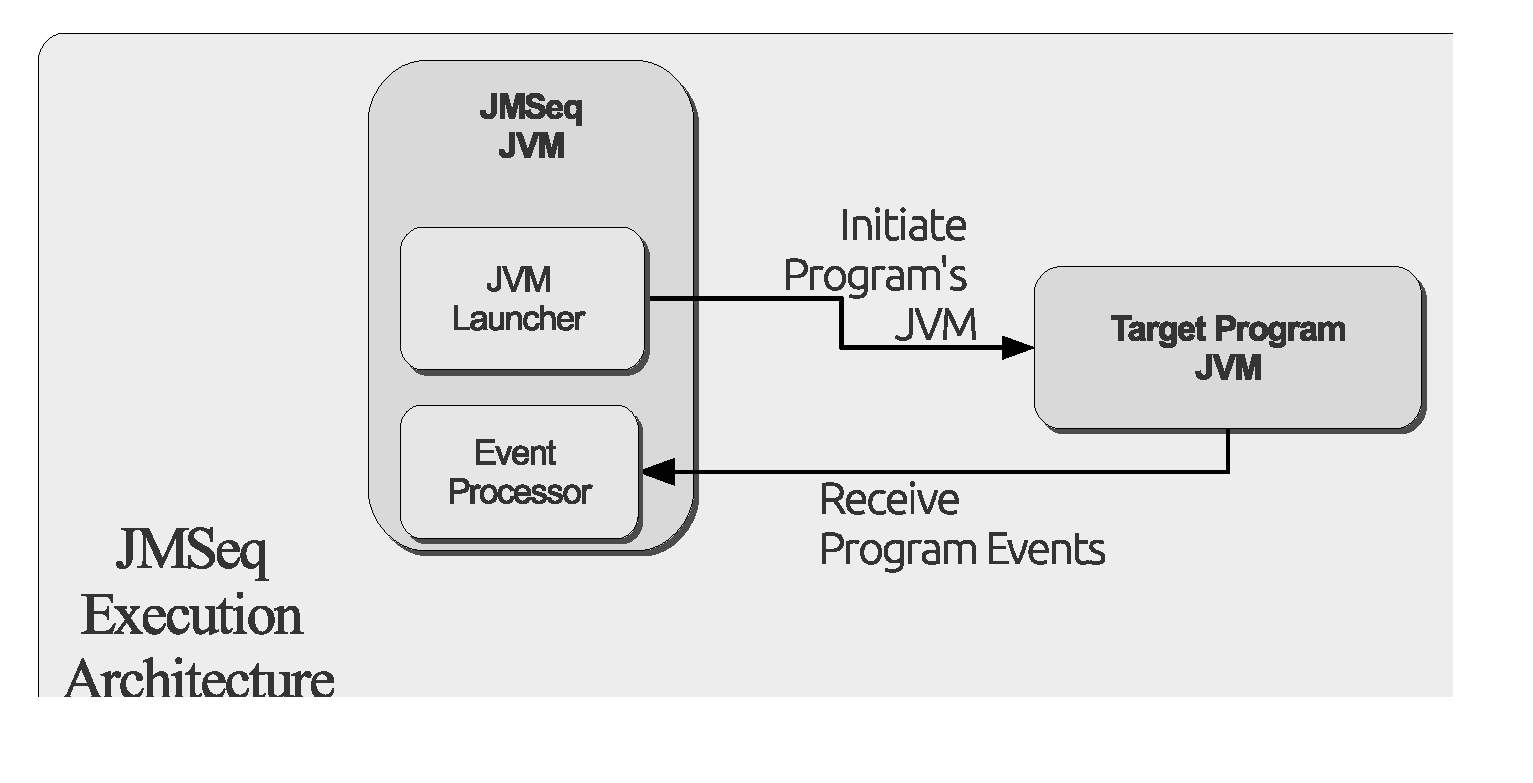
\includegraphics[scale=0.5]{images/arch-diagram-summary-exec}
\caption{JMSeq Execution Architecture}
\label{ch05:fig:arch-overview}
\end{center}
\end{figure}

In this paper, we introduce JMSeq, a tool for monitoring  sequences of method calls in Java programs.
JMSeq is based on Java annotations rather than (source code or bytecode) instrumentation. 
%, at source or bytecode level, we use another approach, called JMSeq.
%JMSeq monitors  sequences of method calls using.
Therefore, it does \emph{not} require  access to the source code of the target application.
JMSeq detects the annotated methods from the target application at runtime. 
Furthermore,  Java annotations themselves have no direct effect on program execution or logic of the application;
they carry metadata that can optionally be used at runtime to perform operations orthogonal to the execution of the main application.
   %Annotations are based on a declarative language to specifiy method call sequences using regular expressions for method signatures.
%The program is verified against the specifications during runtime and fails as soon as a violation is detected. 
%The verification is performed in a separate virtual machine to protect the original application from any modification (Figure \ref{ch05:fig:arch-overview}). 
%In the following, we provide a  discussion of what distinguishes JMSeq from other related work (c.f. Section \ref{ch05:sec:relworks}) in verification:
The main distinguishing overall characteristic of JMSeq is
the integration of the following main features.

\begin{description}
%   \item[Specification language.] JMSeq introduces a simple declarative specification language.
%   The programmer can use the language to express verification requirements using simple expressions from the language.
%   The language is based on regular expressions of method call signatures.
%   The language is simple and intuitive to help the programmer identify different types of sequences of method calls.
   \item[Java annotations.] 
%JMSeq uses Java annotations to specify and verify the sequence of method calls. 
JMSeq annotations specify  method call sequences  in terms of regular expressions of method call signatures.
 This pure declarative language is simple and intuitive in  specification  of  different types of sequences of method calls.
   \item[JVM decoupling.]
To ensure that the target program is in \emph{no} way affected or changed during monitoring, JMSeq runs in a separate JVM from the target application's JVM.
   JMSeq uses Java Platform Debugger API (JPDA) \cite{JPDA_Home} to initiate a separate JVM and verify the target application using events from the target JVM.
  Figure \ref{ch05:fig:arch-overview} displays the high-level execution architecture of JMSeq.
   \item[Fail-fast approach.] JMSeq terminates execution as soon as a violation of a specification occurs.  This approach prevents unsafe behavior,
   enables the localization of an error, and facilitates a reaction
   to a failure immediately, thus making the software more robust~\cite{Shore04a}.
   %In mission-critical software, this approach is favored over others because it facilitates a reaction to the situation as soon as it occurs.
   %It helps the software/service provider to be able to provide better software to its end users.
   %It additionally contributes to better disaster recovery of software in failure situation.
\end{description}


An important consequence of these features
is that neither  the source code (even if available) nor bytecode is modified by JMSeq. 
Furthermore,  JMSeq does not require source code to be present.  
As such, JMSeq is suited for
the specification and verification of both
 newly built software and legacy systems, including third-party libraries
(and even the Java standard library).
For example, given  the API of a legacy system, its expected behavior  can be
specified by annotating the methods of a ``driver'' program which triggers
the legacy code.
JMSeq then verifies the triggered behavior of the legacy code using these
annotations.
%
%   In the context of legacy systems, it can be assumed that the sequence of API and method calls are known.
%   It is also known that JMSeq annotations are not placed on the legacy system.
%   This means that a helper program is needed to use the annotations from JMSeq.
%   Therefore, one can write a helper program that uses the legacy system and its API.
%   The helper program is annotated with JMSeq annotations.
%   Then, the helper program is executed through JMSeq.
%   JMSeq verifies the legacy system through the helper program that carries the annotations and as such the specification of method call sequences from the legacy system.
%   JMSeq verification of legacy system is distinguished from approaches that use instrumentation (especially source level) because access to source code cannot be presumed.
 In the context of an ongoing software development process, JMSeq can also be used as mentioned above
by means of a ``driver'' program but also by directly
annotating the ``interfaces'' of the system API.
%   Since Java annotations have no effect on the execution of the application, they behave as metadata at runtime.
%   JMSeq can detect them and verify the system without the need for a helper program.
By annotating the  interfaces of a system any service object that implements the interface behavior inherits the annotations and can be verified by JMSeq.
In this  respect, JMSeq also introduces integration with frameworks such as JUnit (cf. Section \ref{ch05:sec:junit}). 



The rest of the paper is organized as follows.
The first three sections describe the usage of JMSeq.
Section \ref{ch05:sec:spec} presents the language for specifying sequences of method calls, 
and Section \ref{ch05:sec:impl_annot} discusses the types of annotations available in JMSeq.
These two sections are connected via examples in Section \ref{ch05:sec:samples}.
Afterwards, implementation of the JMSeq framework is explained in detail in Section \ref{ch05:sec:implementation}.
The practical applicability of JMSeq is demonstrated by means of a case study from industry in Section \ref{ch05:sec:frh} and performance evaluation in Section \ref{ch05:sec:results}. 
Finally, related work is discussed in Section \ref{ch05:sec:relworks}.
Section \ref{ch05:sec:conclusion} concludes the paper. %discuss possible future work.

\section{Method Call Sequence Specification} \label{ch05:sec:spec}

We consider a component to be a collection of compiled Java classes. The
relevant dynamic behavior of a component can be expressed in terms of specific
sequences of messages among a small, fixed number of objects. In
Figure \ref{ch05:fig:seq-spec}, we see two UML message sequence diagrams each
describing how, and in which order, the four objects interact with each other. In this
section, we develop a specification language for describing these kinds of
interactions.
 
%Many approaches use finite state machines or regular
%expressions to specify sequences of method calls, and as such it cannot be
%applied to specify recursive call-backs.

%A vertical line is associated
%to each object, representing its lifetime (from top to bottom). The solid
%horizontal arrows are labeled by a method name and represent calls, whereas the
%dashed arrow are return messages. 

In addition to specifying the order, a specification language for sequences of method calls
needs to distinguish between the following two cases (depicted in
Figure \ref{ch05:fig:seq-spec}).
\begin{description}
  \item[Case $1$] 
  shows a scenario in which (the call to) \texttt{m\_c} is nested in 
  \texttt{m\_b} since \texttt{m\_c} is called during the activation of 
  \texttt{m\_b} (i.e., after \texttt{m\_b} is called and before it returns). 
  Similarly, both \texttt{m\_b} and \texttt{m\_c} are nested in \texttt{m\_a}.
  
  %exemplifies a nested method call in which methods from
  %different/same objects are called in a nested way creating new instances of
  %stack trace in the program execution. More specifically,
  %method call to \texttt{m\_c} is nested in method call to \texttt{m\_b} that in
  %turn is nested in method call to \texttt{m\_a}.
  
  \item[Case $2$] represents a method call in which methods from
  different/same objects are called in a sequential rather than nested
  manner. In this example, both \texttt{m\_b} and \texttt{m\_c} are called by
  \texttt{m\_a}.
\end{description}
Typically, a program will need a combination of both cases to specify its dynamic behavior.
Specifying only the order of the method calls is not enough, as both cases above
have the same order of method calls. It is thus required to have a specification
technique that distinguishes between the \textsl{method calls} and
\textsl{method returns}. \begin{figure}[h]
\begin{center}
  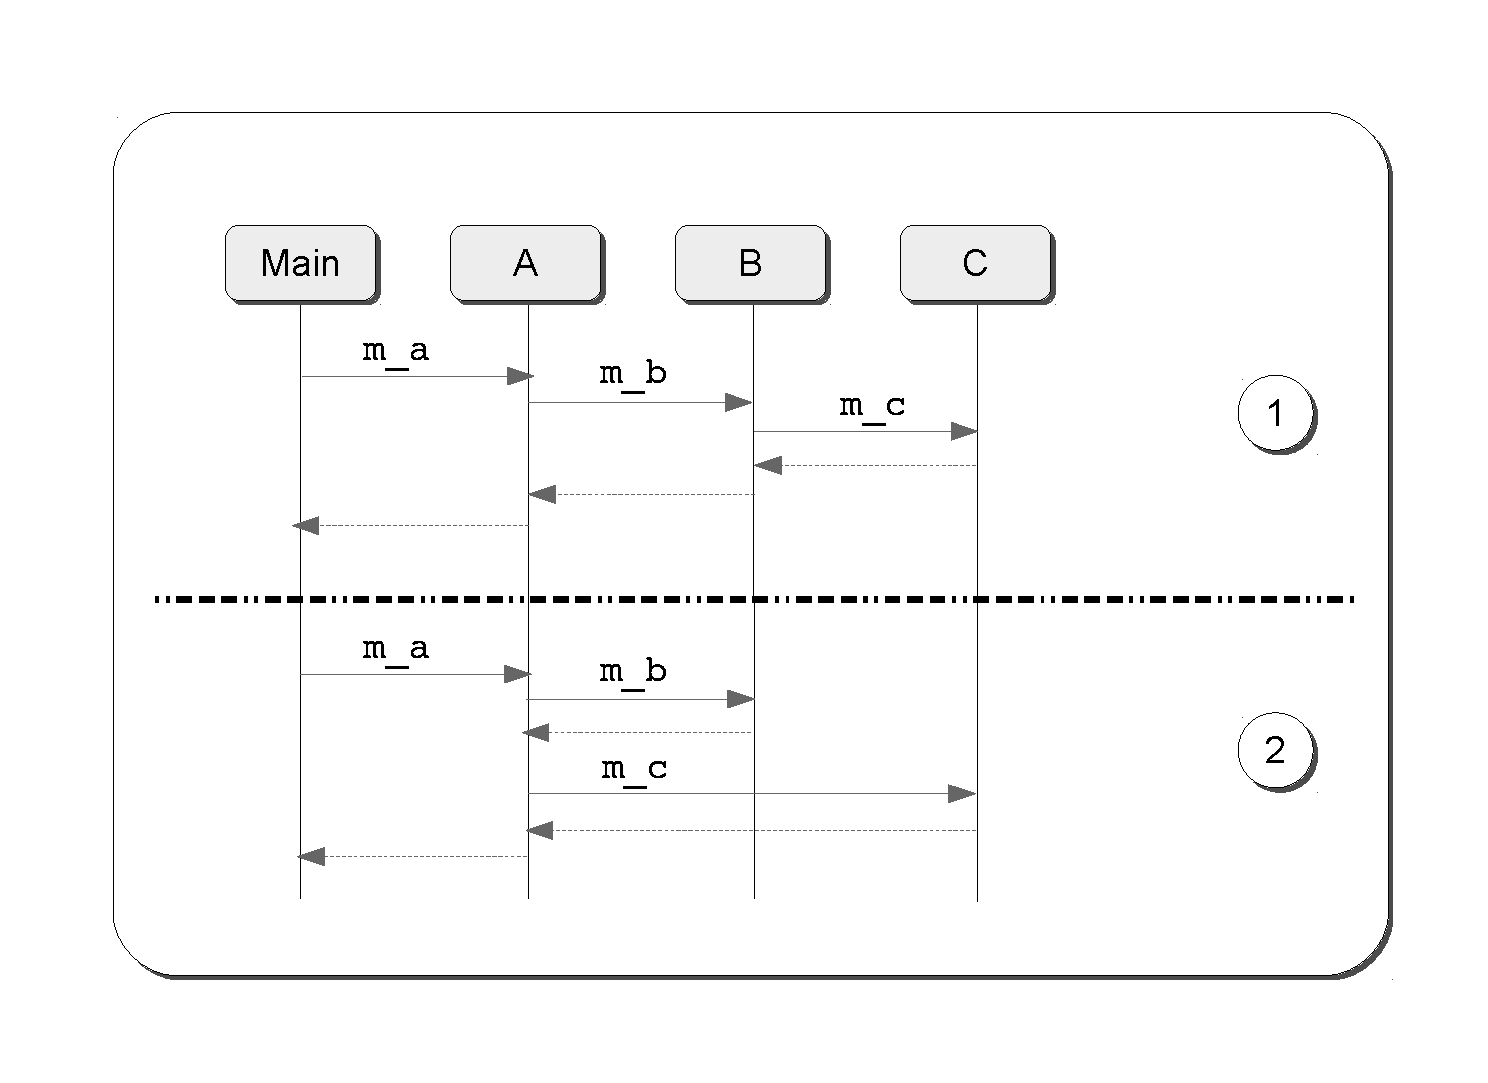
\includegraphics[scale=0.4]{images/seq-spec}
  \caption{Examples of Method Call Sequence Specification}
  \label{ch05:fig:seq-spec}
\end{center}
\end{figure}

%It is clear from the above examples that regular expressions over method calls
%are not enough to specify the typical nested call structure of a sequence of
%messages in the presence of recursion. In general, such sequences form a
%context free language. However they have a special structure: there is a
%deterministic pushdown automaton accepting them such that it pushes or pops at
%most one symbol only, depending if a method call or return is read,
%respectively. Such an automaton is called a visibly pushdown
%automaton \cite{Alur_abstractvisibly}.
 
 
% TODO: mention that events are always accepted for the same object for a single
% method activation

In JMSeq, a specification is written as a post-condition associated with a method. It
specifies the set of possible sequences of method calls, or protocol, of an
object in the context of the relevant part of its environment. Formally,
sequences of method calls can be specified by means
of the grammar in  Figure \ref{ch05:fig:spec_grammar}.

\begin{figure}[h]
\begin{center}
\begin{framed}
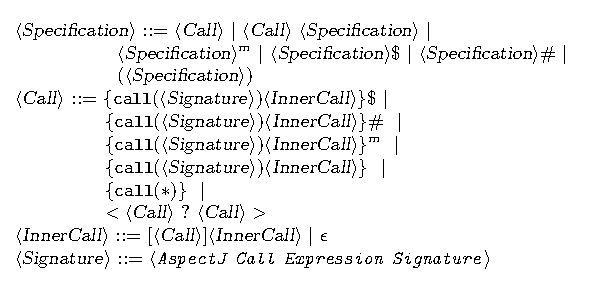
\includegraphics[scale=1]{grammar}
\end{framed}
\caption{Method Sequence Specification Grammar}
\label{ch05:fig:spec_grammar}
\end{center}
\end{figure}

A \textsl{specification} consists of a sequence of calls that can be repeated an
a priori fixed number of times 
("${\langle}$\textsl{Specification}${\rangle}^m$"), with $m \geq 0$, one or
more times ("${\langle}$\textsl{Specification}${\rangle}\$ $"), or zero or more
times ("${\langle}$\textsl{Specification}${\rangle}\#$"). Although JMSeq does
not use aspect-oriented programming in its implementation, we have used the
generic method call join points syntax of AspectJ \cite{kiczales_aspectj},
using for example $\#$ to denote the more standard Kleene star operation.
Additionally, $(\langle$\textsl{Specification}$\rangle)$ is a way to group
specifications to avoid ambiguity. To improve readability of the
specifications, grouping is only used when necessary.

A \textsl{call} is a call signature followed by a (possibly empty) sequence of
inner calls. Each call can be repeated either one or more times, zero or more
times, or exactly $m$-times, for some $m \in \{1, 2, 3, \ldots \}$;
i.e., $m$ is a constant. 
Having the repetition by $m$ does not make the language go beyond the expressiveness of regular expressions.
Additionally, the wild card 
{\small$\{$\textbf{\texttt{call}}$(*)\}$} denotes a call to an arbitrary method.
To support branching, JMSeq also provides
$<\langle$\textsl{Call}$\rangle ? \langle$\textsl{Call}$\rangle>$ to allow the
specification of a choice in a sequence of method executions.

\textsl{Inner calls} are calls that are executed before the outer
call returns, i.e., they are nested. 
We do not have explicit return messages, but rather we specify the scope of a call  using brackets. 
Information about the message call, like the type of the caller and the callee, method
name, and the types of the parameters are expressed using a syntax similar to that of AspectJ. 
Simply put, a call signature is of the form
\begin{alltt}
\small
\texttt{call}([ModifiersPattern] TypePattern
        [TypePattern . ] IdPattern (TypePattern | ".." , ... )
        [ throws ThrowsPattern ]
)
\end{alltt}
reflecting the method declarations in Java.
The two leftmost patterns specify the method modifiers (like   ``static'' or ``public'') and return types.
% that include method names, method
%parameters, return types, modifiers, and throws
%clauses. 
Here \texttt{IdPattern} is a pattern specifying the method name. It can possibly
be prefixed at the left by a specification of the type of the object called.
The method name is followed by a specification of the types of the parameters
passed during the call, and possibly by a specification of the exceptions that may be thrown.
It implies that JMSeq specification grammar can distinguish the overloaded
methods in a class. Patterns may contain wild card symbols ``\texttt{*}'' and
``\texttt{..}'', used for accepting any value and any number of values,
respectively. For example, the call
\begin{alltt}
\centering\small
\texttt{call(* *.A.m\_a(..))}
\end{alltt}
is denoting a call to method \texttt{m\_a} of any object of type \texttt{A}
that is placed in any package, and returning a value of any type. If there is a
need to be more specific, a possible restatement of the same specification
could be:
\begin{alltt}
\centering\small
\texttt{call(int nl.liacs.jmseq.*.A.m_a(Object, double))}
\end{alltt}

Next we give a few examples of correct method sequence specifications. 
For instance, the specification of the sequence in case $1$ of
Figure \ref{ch05:fig:seq-spec} is given by:
%\begin{flushleft}
%\includegraphics[scale=1]
\begin{alltt} 
\centering\small{\color{red}\{}call(* *.A.m_a(..)){\color{red}[}{\color{blue}\{}call(* *.B.m_b(..)){\color{blue}[}\{call(* *.C.m_c(..))\}{\color{blue}]}{\color{blue}\}}{\color{red}]}{\color{red}\}}
\end{alltt}

%\end{flushleft}
%\begin{alltt}
%\centering\small
%{\color{red}\{}call(* *.A.m_a(..)){\color{red}[}{\color{blue}\{}call(*
%*.B.m_b(..)){\color{blue}[}\{call(*
%*.C.m_c(..))\}{\color{blue}]}{\color{blue}\}}{\color{red}]}{\color{red}\}}
%\end{alltt}
Here it is important to notice that the call to method  \texttt{m\_b} is internal
to \texttt{m\_a}, and the call to \texttt{m\_c} is internal to \texttt{m\_b}.
The sequence in case $2$ of the same figure would be:
%\begin{flushleft}
%\includegraphics[scale=1]
\begin{alltt} 
\centering\small{\color{red}\{}call(* *.A.m_a(..)){\color{red}[}\{call(* *.B.m_b(..))\}{\color{red}]}{\color{red}[}\{call(* *.C.m_c(..))\}{\color{red}]}{\color{red}\}}
\end{alltt}

%\end{flushleft}
%\begin{alltt}
%\centering\small
%{\color{red}\{}call(* *.A.m_a(..)){\color{red}[}\{call(*
%*.B.m_b(..))\}{\color{red}]}{\color{red}[}\{call(*
%*.C.m_c(..))\}{\color{red}]}{\color{red}\}}
%\end{alltt}
where both calls to methods  \texttt{m\_b} and \texttt{m\_c} are internal to
\texttt{m\_a}.

These two cases depict a fixed sequence of method calls. More interesting are the cases when,
for instance, the method \texttt{m\_a} should be called at least once before any possible
method call to \texttt{m\_b} or \texttt{m\_c}:
%\begin{flushleft}
%\includegraphics[scale=1]
\begin{alltt} 
\centering\small\{call(* *.A.m_a(..))\}\${\color{red}<}\{call(* *.B.m_b(..))\}\#{\color{red}?}\{call(* *.C.m_c(..))\}\#{\color{red}>}
\end{alltt}

%\end{flushleft}
%\begin{alltt}
%\centering\small
%{\color{red}\{}call(* *.A.m_a(..)){\color{red}\}}\${\color{red}\{}call(*
%*.B.m_b(..)){\color{red}\}}\#
%\end{alltt}

Such a specification is used in circumstances where the execution of  \texttt{m\_a} is a prerequisite to the execution of either of \texttt{m\_b} or \texttt{m\_c}.
% 
% It is \emph{notable} that the meta-grammar provided in Figure
% \ref{ch05:fig:spec_grammar} is a context-free grammar; 
It is notable that the actual specifications are regular expressions;
for example, they may contain  unbounded repetitions and a choice of calls.

\section{Annotations for method call sequences} \label{ch05:sec:impl_annot}
Java enables developers to attach extra metadata to their programs using annotations.
%Java provides a means to annotate parts of a program.
These metadata do not directly affect the program semantics, but they do affect the
way programs are treated by tools and libraries, which can in turn affect the
behavior of the running program \cite{Java_5_Annotations}. Annotations can be
read from source files, class files, or reflectively at runtime. 
One can define custom annotation types and use them to provide the desired types of metadata for the declarations in his program. 
In Java, an annotation is a special kind of modifier, and can be used anywhere other
modifiers (such as {\small\texttt{public}}, {\small\texttt{static}}, or
{\small\texttt{final}}) can be used.

We use annotations as an enabling feature to test components without the need to have their source code.
We only use the metadata loaded from the annotations during runtime.
These metadata include the specification of the sequences of method calls
based on the grammar discussed in Section \ref{ch05:sec:spec}. The metadata
is placed on classes or methods in a Java program. 
Then, they are loaded into JMSeq when it monitors the actual observable
behavior of the program at runtime.

JMSeq defines two type of annotations: sequenced object annotations and
sequenced method annotations.

\subsection{Sequenced Object Annotations}

To verify the sequence of executions, methods in classes need to be
annotated. Thus, JMSeq needs to detect all  classes that contain
some method carrying an annotation for verification. 
To improve readability and performance, JMSeq introduces
\smalltt{SequencedObject} annotation. This annotation is a marker
for such classes and notifies the annotation metadata loader (cf.
Section \ref{ch05:sec:annotation_repo}) that the objects instantiated from the annotated
class contain methods that specify a sequence of method executions. 
The code is given in Listing \ref{ch05:lst:seq_obj}.


\lstset{language=Java}
\begin{lstlisting}[label=lst:seq_obj, caption=SequencedObject Annotation Declaration]
@Retention(RetentionPolicy.RUNTIME)
@Target(ElementType.TYPE)
public @interface SequencedObject {
   // we need no properties for this annotation as this is only a marker.
}
\end{lstlisting}

In Listing~\ref{ch05:lst:seq_obj}, {\small\texttt{@Retention(RetentionPolicy.RUNTIME)}} declares that this
annotation is only applicable during runtime and may  not be used in other scenarios.
Moreover, {\small\texttt{@Target(ElementType.TYPE)}} declares that this
annotation can only be used on types including classes, interfaces and
enumerated types; in other words, this annotation may not be used to mark a method
in a Java class.

\subsection{Sequenced Method Annotations}
A sequenced method annotation is used to specify the sequences of method
calls beginning from a given method. The annotation requires a string
property declaring the sequence specification discussed in Section
\ref{ch05:sec:spec}. Listing \ref{ch05:lst:seq_method} presents the declaration of
this annotation type.

\lstset{language=Java}
\begin{lstlisting}[label=lst:seq_method, caption=SequencedMethod Annotation Declaration]
@Retention(RetentionPolicy.RUNTIME)
@Target(ElementType.METHOD)
public @interface SequencedMethod {

   String value();

   boolean allowExceptions() default true;

   Class<?>[] expect() default {};

   Class<VerificationFailureHandler> verificationFailureHandler();
}
\end{lstlisting}

{\small\texttt{@Target(ElementType.METHOD)}} declares that this annotation is
only applicable to \textit{methods}. The string value from
{\small\texttt{value()}} holds the sequence specification (cf.
Section \ref{ch05:sec:spec}). 
Additionally, a sequenced method annotation allows verification of
exceptions during runtime. The tester can configure whether exceptions
are allowed or not using the combination of \smalltt{allowExceptions()}
and \smalltt{expect()}:
\begin{description}
  \item[\smalltt{allowExceptions()=true}] implies that exceptions are allowed during execution; 
  this is the default case.
If there is no exception configured using \smalltt{expect()},
\emph{any} exception is acceptable; otherwise,  an exception is acceptable 
only if it is specified in the array
of classes in \smalltt{expect()} or if it is a subclass of one of them.
If an exception occurs and it is ``expected'', JMSeq allows the program to continue execution;
the program should nevertheless be able to properly deal with the exception.

  \item[\smalltt{allowExceptions()=false}]  means that no exceptions are
expected during the execution. In this case, the value specified by
\smalltt{expect()} is ignored.
\end{description}

JMSeq additionally provides a general mechanism to specify how to handle situations in
which the sequenced execution fails to complete. This can happen
because of a method call which was not included in the specification, or
an unexpected exception.
To this end, JMSeq introduces \smalltt{Verification\-FailureHandler} interface as an
extension point where the tester or developer can provide 
custom behavior to gracefully deal with the verification failure.
This interface
introduces a single method: \smalltt{handle\-FailedExecution(Execution
e)}. 
This method
%\smalltt{handle\-FailedExecution(Execution e)} 
receives information about the execution through a parameter of
type \smalltt{Execution} (cf. Section \ref{ch05:sec:implementation}).
\smalltt{Execution} is the central data model that carries information
about the method execution sequences; the trail of the
executions may be useful to the developer to examine the failure causes.
%
If no such handler is provided, verification failure results in termination 
of program execution with a failure status.

Section \ref{ch05:sec:samples} provides more discussion along with different
examples on using JMSeq.

\section{JMSeq by example} \label{ch05:sec:samples}
In this section, we go through different usage scenarios of JMSeq 
by means of illustrative examples.

\subsection{Sequenced Execution Specification}
In  Listing \ref{ch05:lst:annotated_spec}, we again go through the example
introduced in Section \ref{ch05:sec:spec}.
% give two examples of
% annotations of the class {\small\texttt{Main}} in Figure
% \ref{ch05:fig:seq-spec}. 
In this example, we annotate the method \texttt{main()} with the sequences of method calls describing the two scenarios
given in Figure \ref{ch05:fig:seq-spec}. 
The JMSeq specifications used here are discussed in Section \ref{ch05:sec:spec}.
The listing shows how to use them in a Java program.

\lstset{language=Java}
\begin{lstlisting}[label=lst:annotated_spec, caption=Sample annotated specification]

// Case 1
@SequencedObject
public class Main {

   @SequencedMethod(
     "{call(* *.A.m_a(..))[{call(* *.B.m_b(..))" + 
     "[{call(* *.C.m_c(..))}]}]}") 
   public void main() { 
      // ...
   }
   
   public void init() {
      // ...
   }
}

// Case 2
@SequencedObject
public class Main {

   @SequencedMethod("{call(* *.A.m_a(..))" + 
     "[{call(* *.B.m_b(..))}][{call(* *.C.m_c(..))}]}") 
   public void main() {
      // ...
   }
   
   public void init() {
      // ...
   }
}
\end{lstlisting}

\subsection{Exception Verification}
We discuss how JMSeq can be used to verify  occurrence of exceptions during
execution of an application using the example given in Figure
\ref{ch05:fig:seq-spec} Case 1.

Let's assume that \smalltt{m\_c} may encounter
\smalltt{NullPointerException} and \smalltt{m\_b} may face
\smalltt{IOException}. But, we do not hold any assumption on the
location in the code where the exceptions may be handled or even
totally ignored. We use the following annotation in Listing
\ref{ch05:lst:case-1-exceptions} to express this situation.

\lstset{language=Java}
\begin{lstlisting}[label=lst:case-1-exceptions, caption=Exception
Specification for Case 1]
// Case 1
@SequencedObject
public class Main {

   @SequencedMethod("{call(* *.A.m_a(..))" + 
     "[{call(* *.B.m_b(..))[{call(* *.C.m_c(..))}]}]}",
     allowExceptions = true,
     expect = {NullPointerException.class, 
               IOException.class}) 
   public void main() { 
      // ...
   }

}
\end{lstlisting}

During the execution of the application, if any exception occurs,
JMSeq receives the event of the exception occurrence. Since exceptions
are allowed, there will be no verification failure by JMSeq as long as
the exceptions received and verified are either instances of the
specified exception classes or any of their subclasses.
However, if the underlying application does not handle the exceptions
(i.e., proper use of \smalltt{try/catch}), they are
propagated up in the call stack and this may result in JVM crash.
%because of the application ignorance of the exceptions. 

For instance, if an instance of \smalltt{FileNotFoundException} occurs
in \smalltt{m\_c}, JMSeq accepts the exception (because it is a subclass of
\smalltt{IOException}) and allows the application to continue. If the
application at some point deals with the exception, the execution
continues; otherwise JVM stops, complaining that the exception is not handled.
On the other hand, if an \smalltt{IllegalStateException}
happens during the execution of the program, JMSeq does not allow the
application to receive the exception since it is not one of the expected
exceptions in the specification. 
Instead, it runs the failure code provided by the tester (if any).

In another situation in Case 1, assume that \emph{no} exceptions are
acceptable during the execution. For this to happen, we simply use
\smalltt{allowExceptions = false} in the specification annotation. In
this case, no exception should occur during the execution of the
application; otherwise JMSeq issues a verification failure. Besides,
when no exceptions are allowed, using \smalltt{expect()} has no effect
on JMSeq verification behavior.

JMSeq additionally supports integration with testing frameworks such as JUnit. 
An example of such integration is discussed in Section \ref{ch05:sec:junit}.

\section{The JMSeq framework} \label{ch05:sec:implementation}

In this section, we present the JMSeq monitoring and verification framework and discuss its implementation, which uses Java $5$ Annotations \cite{Java_5_Annotations} and Java Platform Debugger API \cite{JPDA_Home}. 
More implementation details, including examples and documentation, can be found at \url{http://github.com/nobeh/jmseq}.

As discussed above, to use JMSeq, it is assumed that Java components are supplied with sequenced object and sequenced method annotations. 
Multiple annotations are possible within the same class, but not for the same method. 
This implies that a component specification is in fact scattered across its constituent classes, each of which with a local and partial view of the component behavior.
Only the annotated methods will be monitored by JMSeq.
The overall verification process in JMSeq is depicted in Figure \ref{ch05:fig:alg-verify}.

\begin{figure*}[t]
\begin{center}
  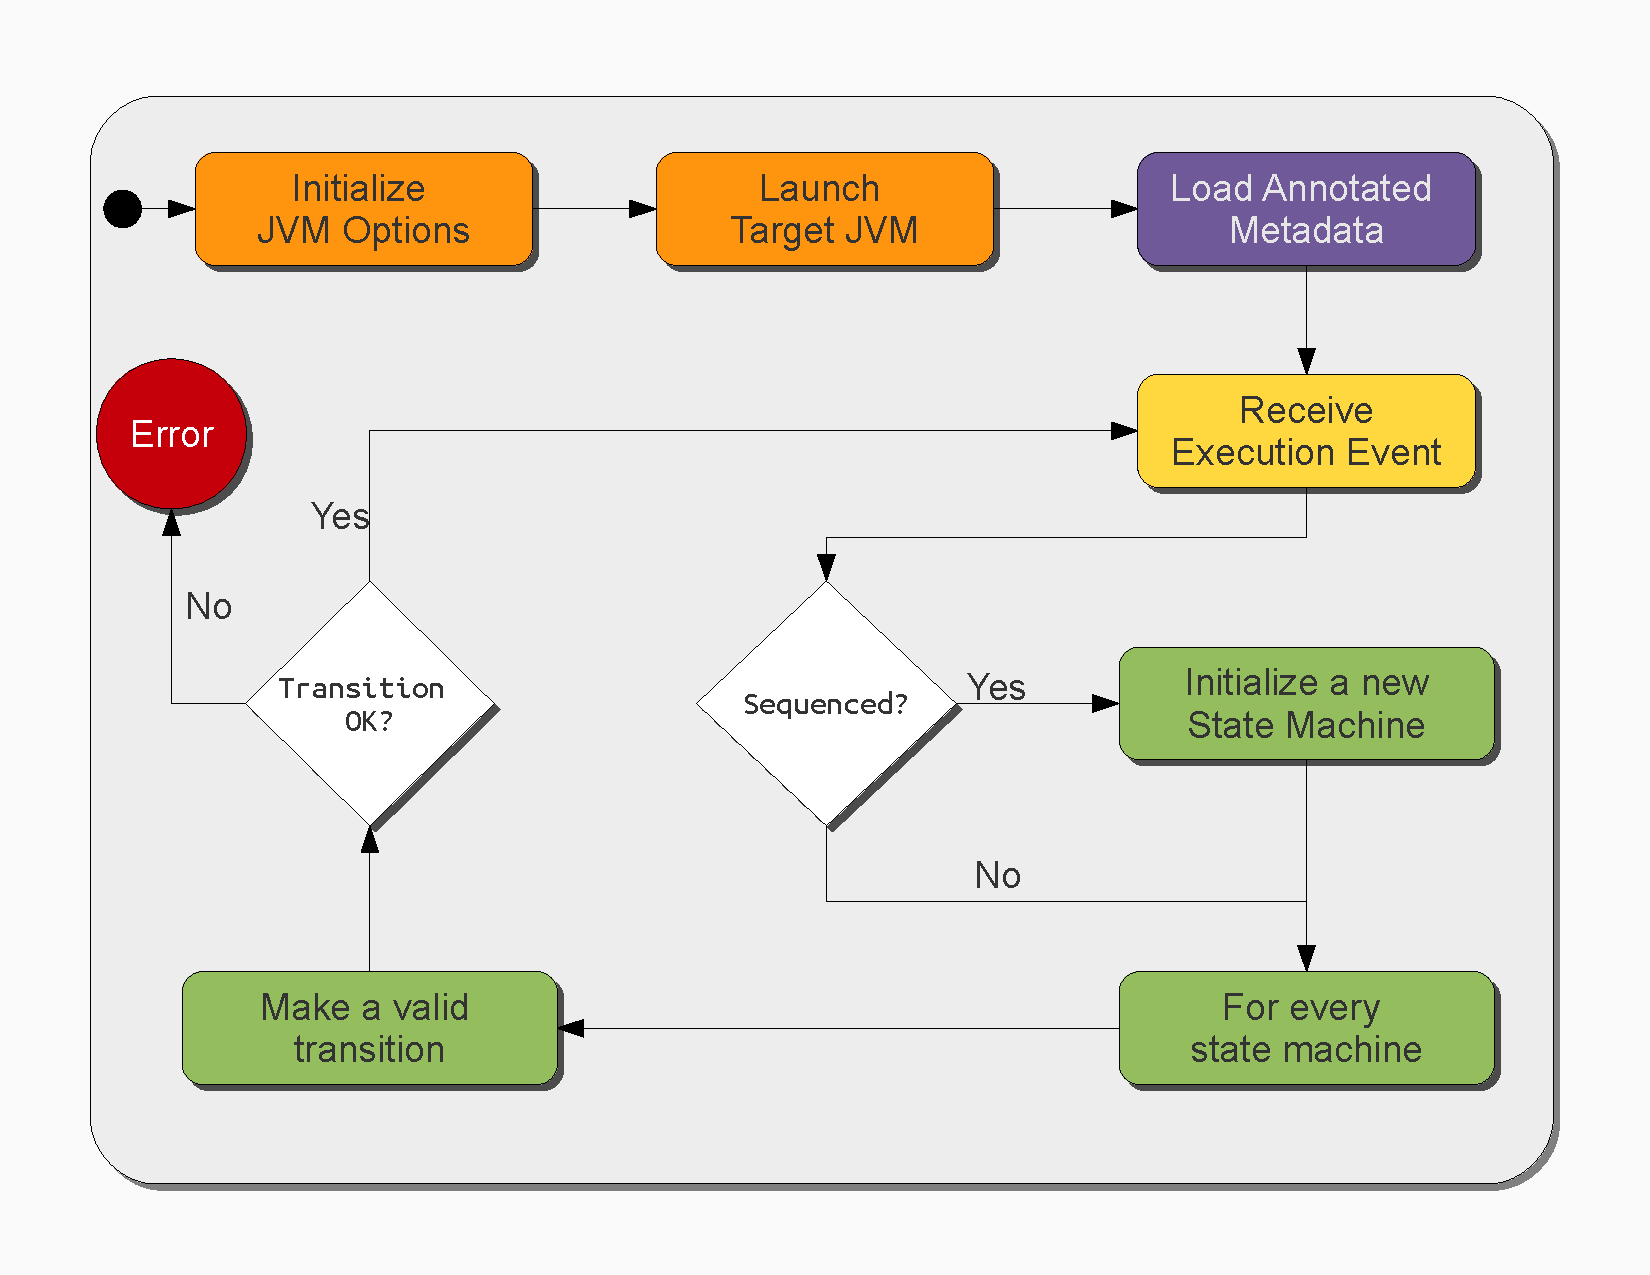
\includegraphics[scale=0.47]{images/alg-diagram}
\end{center}
\caption{Overview of JMSeq's process to verify a program}
\label{ch05:fig:alg-verify}
\end{figure*}

As a Java program, JMSeq executes naturally inside a Java virtual machine (JVM); JMSeq additionally initiates another JVM (called the \textsl{Target JVM}) to be able to control the sequenced execution of the target program.
Through initial parameters, the target JVM is configured to report back to JMSeq some events such as method entry and method exit.
Furthermore, JMSeq does not verify events from all objects but only those specified in these parameters. 
The target JVM takes advantage of the Java Platform Debugger Architecture (JPDA) to access the needed details on the execution of the application while it is running. 

Before verification starts, JMSeq inspects the classes in the execution class path searching for methods that are annotated for sequenced verification; during this process, it collects all of the available method call sequence metadata. 
This step (denoted as Load Annotated Metadata in Figure \ref{ch05:fig:alg-verify}) does not need the source code, but rather uses the annotations metadata available in the compiled code.

The target program subsequently starts its execution and JMSeq reacts to the events it receives.
JMSeq uses state machines to verify the method calls occurring in an application during runtime.
The state machines are indexed by the pairs of method signature and the callee object; thus JMSeq can uniquely identify the associated state machine.
When JMSeq receives a method execution event, it checks if there is a need to initialize a new state machine for that method execution.
A state machine is initialized if there is no state machine for the current method execution and the method is annotated  \smalltt{@SequencedMethod}.
Then, JMSeq tries to verify the current method execution in the context of all active state machines for other methods.
For every state machine, JMSeq tries to make a valid transition in the state machine. 
Verification will continue if such a transition can be made for all state machines; 
if not, JMSeq stops the execution reporting a violation of the specification. 
% of the outermost specification for the current method is detected.
% When a verification failure is detected, JMSeq stops the execution; if a user defined failure handler is present, it will be executed before termination.

The process of matching method execution events with state machine transitions is done in JMSeq by following these steps:
\begin{enumerate}
  \item %A ``call expression'' is constructed based on the information associated to the received event. 
  First, every event received from the target JVM, together with the information associated to the event, is transformed to an instance of \smalltt{Execution} to capture various details about the execution of a method. 
  Then, at verification time, the instance of \smalltt{Execution} is transformed to an instance of \smalltt{CallExpression} to hold method signature details used by the state machine to make a transition. (Section \ref{ch05:sec:event_handling})
  \item Using the metadata available from the annotations of the methods, then, the   next ``possible call expressions'' of the current state, corresponding to the possible next transitions of the state machine,  are built. (Section \ref{ch05:sec:annotation_repo}, \ref{ch05:sec:exec_verify})
  \item A match making is done between the possible call expressions (state machine transitions) and the   current call expression as the candidate.  
  If a match is found,  the transition is made and the method is  accepted; otherwise, it fails. 
  When a failure occurs, JMSeq will execute the custom verification failure handler that is implemented either as part of
  the component code by the programmer, or externally by the system tester. (Section \ref{ch05:sec:exec_verify})
\end{enumerate}

JMSeq computes the possible call expressions on-the-fly instead of constructing the full state machine in the beginning of the verification process. 
This way it avoids the construction of states in the state machine that are never used in the execution. 
To avoid repeated computations of the same states, JMSeq utilizes dynamic programming techniques such as in-memory object caches. 

\subsection{JMSeq Architecture}

The overall architecture of JMSeq is given in Figure \ref{ch05:fig:arch-diag}. It basically
consists of three main modules: one for handling the events raised by the JVM executing the target program, another module for storing the annotation information, and a third
one to perform the runtime verification.

\begin{figure*}[t]
\begin{center}
  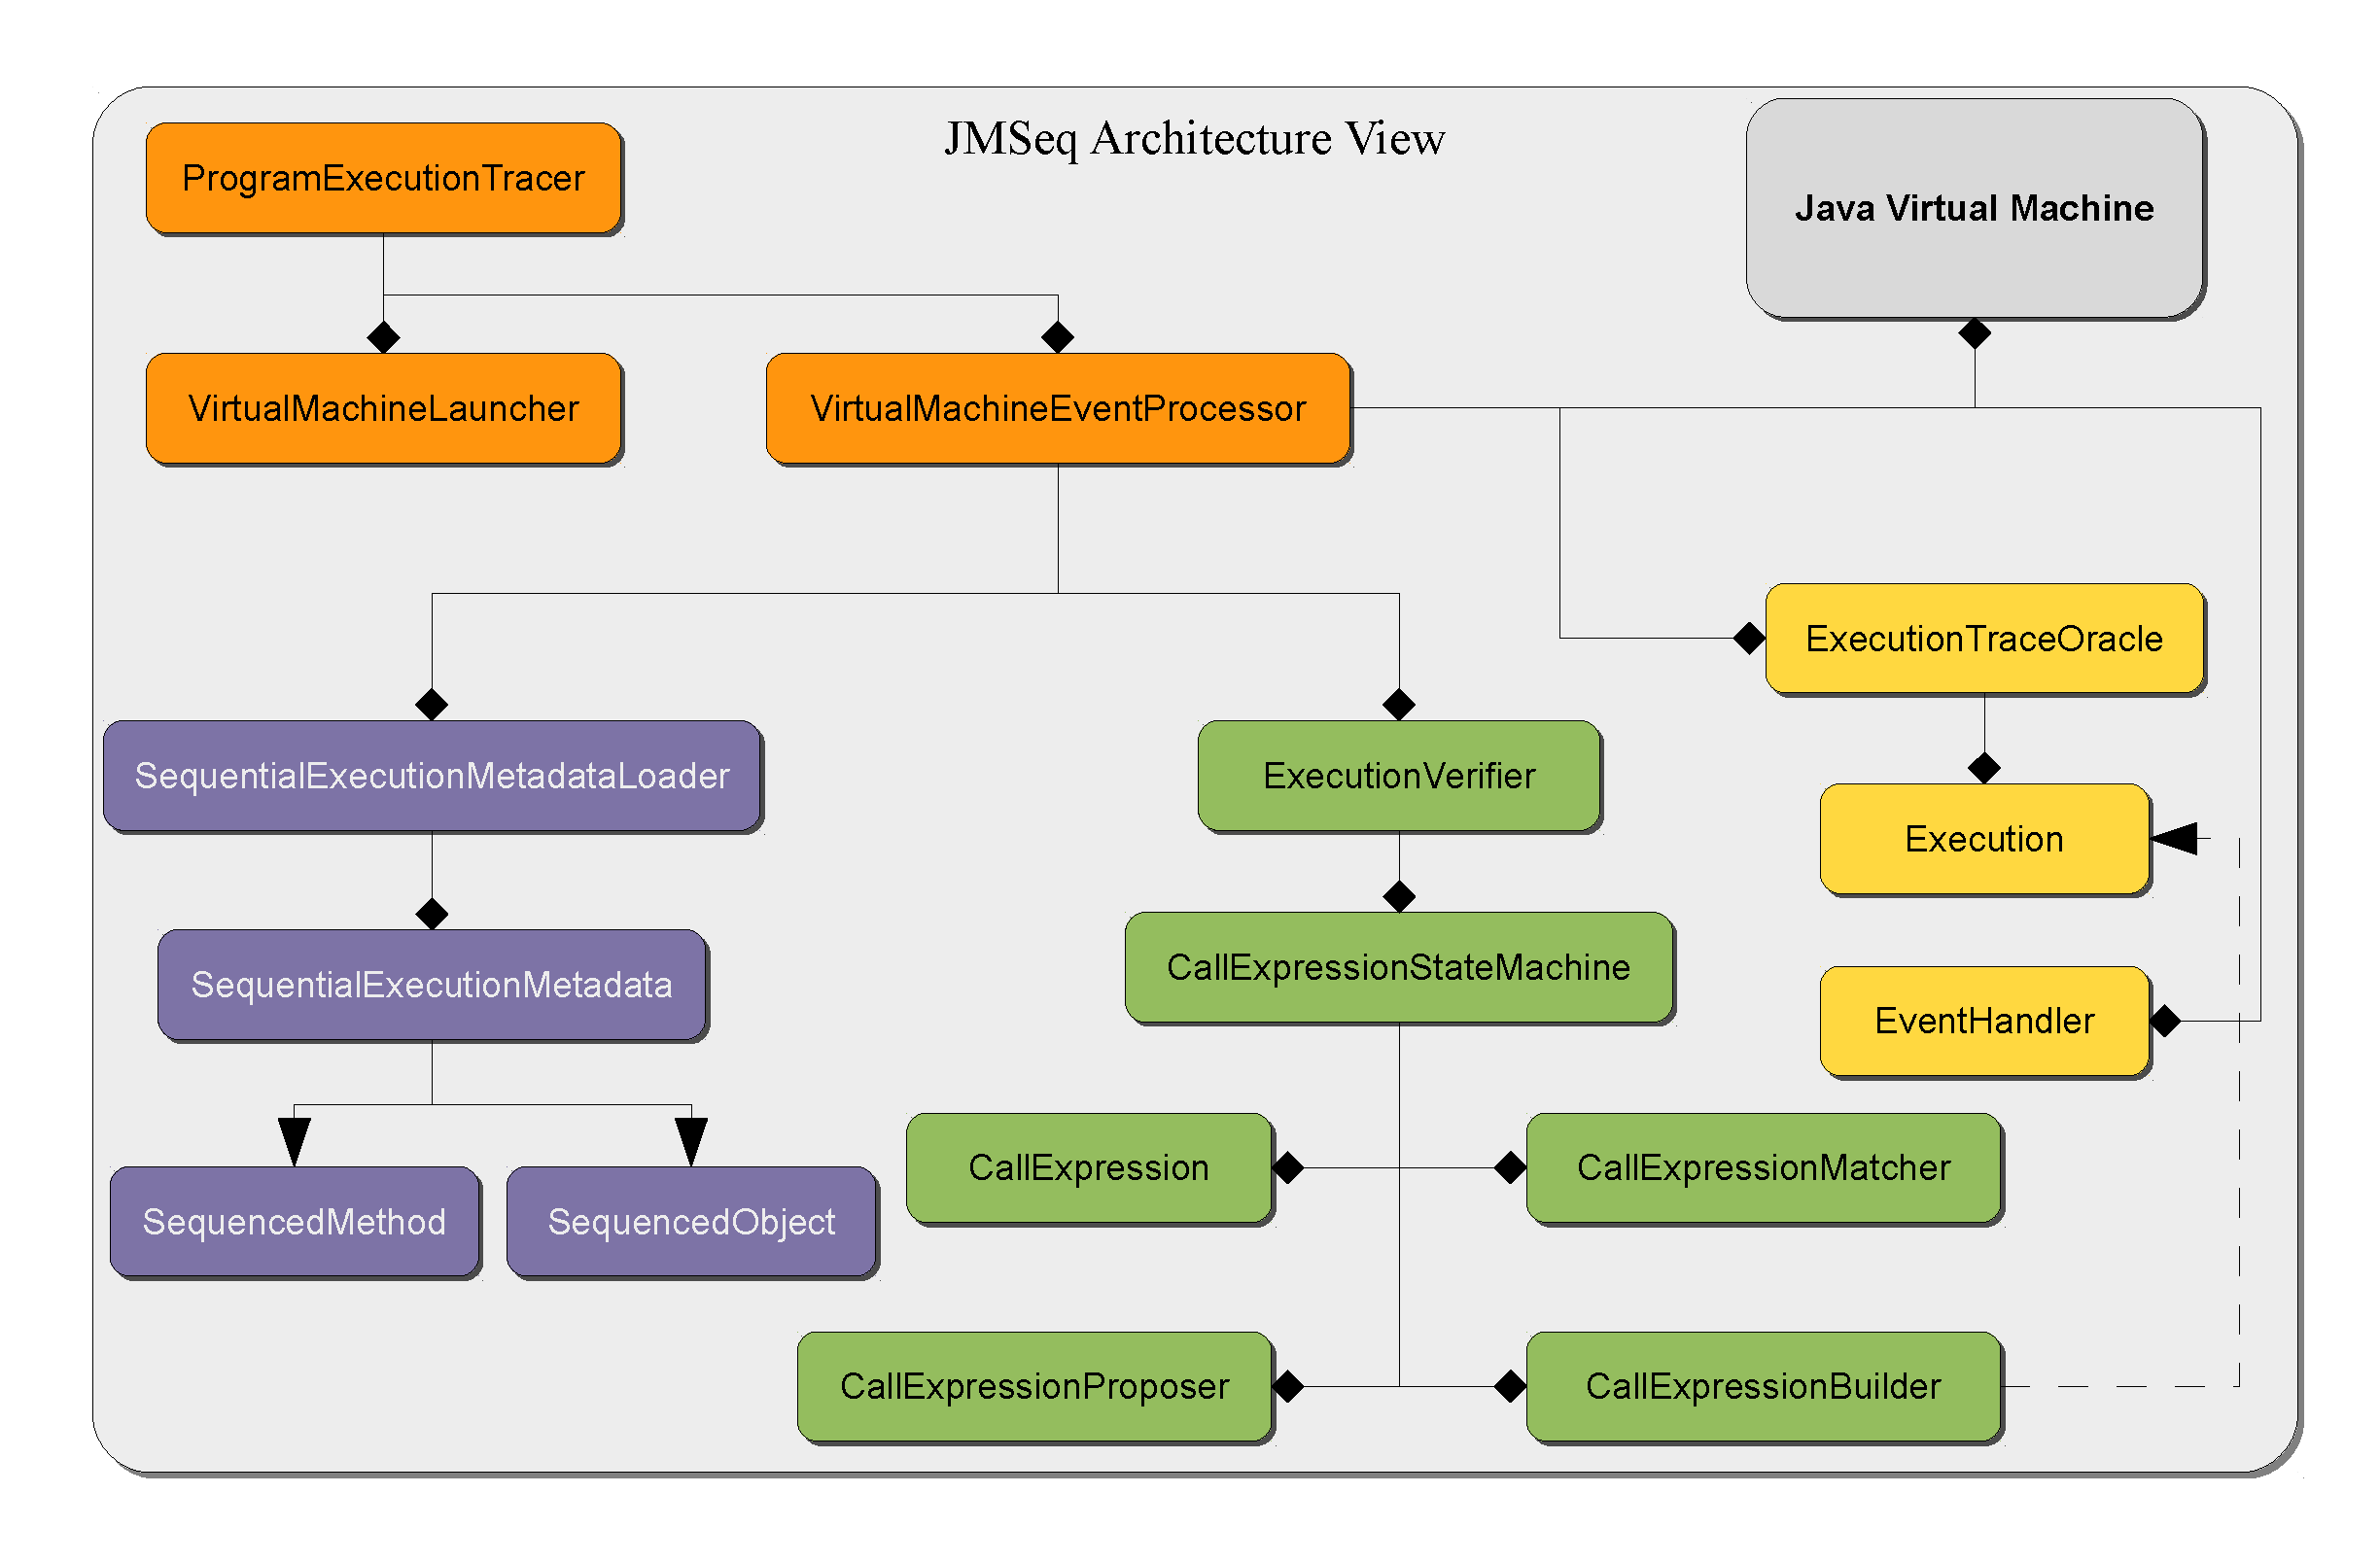
\includegraphics[scale=0.35]{images/arch-diagram}
  \caption{Software Architecture for Method Sequence Specification}
  \label{ch05:fig:arch-diag}
\end{center}
\end{figure*}

% The current design of JMSeq is completely \textsl{general} and \textsl{modular};  as it
% allows for replacing the grammar in Figure \ref{ch05:fig:spec_grammar} with other
% specification modules, based, for example, on temporal logics or extended
% regular expressions.

\subsubsection{Event Handling Module} \label{ch05:sec:event_handling}
Java Debugger Interface (JDI) is the interface
of Java Platform Debugger Architecture (JPDA) that gives access to different details during the execution of a program.
Following the JDI event model, JMSeq takes control over some of the
execution events that JVM publishes during a program execution. Therefore, a
component was designed to model and hold the execution trace events required
for event handling and execution verification.

\begin{enumerate}
  \item \smalltt{Execution} is the central data structure that holds all the
  information about execution that is made available through the JDI event mechanisms.
  Relevant events include ``method entry'', ``method  exit'', and
``exception'' occurrences.
   It provides access to information such as:
   \begin{itemize}
     \item The object that is currently executing (\emph{the callee object}) and
     its unique identifier in JVM.
     \item Event details through subclasses such as method return values or
     \emph{the caller object} reference in case of a method exit event.
     \item \textit{Parent Execution}: every execution can hold a reference to its
     parent execution object forming a directed tree of executions. This helps
     traversing the executions at validation time.
    \end{itemize}
     \item \smalltt{EventHandler} is the event handling interface that
is
     injected into JVM with access to JDI information. The event handler
     receives the events it is subscribed to and possibly takes an associated
     action. In particular it creates an instance of {\small\texttt{Execution}}
     for each sequence annotation and it stores it in the
     {\small\texttt{ExecutionTraceOracle}} registry. In general, all events received and processed by
     {\small\texttt{EventHandler}} are stored in this registry for further use
     by other components, for example, by the
     verification module.
\end{enumerate}

\subsubsection{Annotation Metadata Module} \label{ch05:sec:annotation_repo}

As the execution traces are stored in a repository, they are supposed to be
checked and verified against the formal specifications as described on the
{\small\texttt{@SequencedObject}} and {\small\texttt{@SequencedMethod}} annotations
of the compiled classes in the program. It is the task of the
annotation metadata module to store this information. A small utility
component in this module is responsible to read and load the metadata of all
classes that are annotated. This information is used when there is a
need to verify the conformance of an execution event.

\subsubsection{Execution Verification Module} \label{ch05:sec:exec_verify}

% \note{Most of this paragraph is repetition. If we have time, this repetition can be reduced ideally.}
During execution of a program, those events that need to be monitored are received and
verified against a message sequence specification. 
For every specification in the metadata repository, a state machine is created on the fly.
At each state, JMSeq computes the Brzozowski derivative of the regular expression associated with the current state and memorizes this computation for further use. 
This avoids the full construction of the state machine at each step of verification. 

When a method execution event is received, either the corresponding state machine exists or it should be created.
A state machine is initialized if there is no state machine for the current method execution and the method is annotated  \smalltt{@SequencedMethod}.
JMSeq then tries to verify the event against all active state machines.
For every state machine, an attempt is made to make a valid transition.
If the transition is successfully made, JMSeq continues.
Otherwise, an ``invalid'' transition is detected; verification stops.
At this point, JMSeq checks if an implementation of the
\smalltt{Verification\-Failure\-Handler} interface is present (cf. Section \ref{ch05:sec:impl_annot}).
If present, JMSeq tries to instantiate an instance of the verification failure handler and hands over the execution metadata to this handler. 
Otherwise, JMSeq terminates and reports how the specification is violated.

An event may also be sent due to occurrence of an exception. 
In this case, the execution is verified based on the exception specifications expressed using the mechanism described in Section \ref{ch05:sec:impl_annot}. 
If the exception is allowed and verified the execution continues; otherwise, it fails and control is delegated to verification failure handler as explained above.


The execution verification component is composed of the following elements:
\begin{enumerate}
  \item \textsl{Call Expression} is a simple component for interacting with each
  state machine object. Basically, it transforms execution events coming from
  the JVM into call expressions used by the state machine components.
  \item \textsl{Call Expression State Machine}: Sequences of
  executions are translated to ``call expressions'' that are to be accepted by
  a state machine. The state machine needs to distinguish the
  method's context on different calls to the same method. At the
  end of a successful sequential execution, the state machine associated to that
  sequenced execution specification should be in a success state. 
  \item \textsl{Call Expression Builder} constructs a call expression out of:
  \begin{enumerate}
    \item A string which is in the format of the JMSeq specification grammar as
    in Figure \ref{ch05:fig:spec_grammar}. This service is used the first time a
    sequential execution is detected to build the root of the future possible
    (candidate) call expressions.
    \item An execution event; every time an execution is handed over to the
    verification module, an equivalent  call expression is built for it so
    that it can be compared and matched against the call expression for the
    previous event.
  \end{enumerate}
  \item \textsl{Call Expression Proposer} is a service proposing \textit{possible
  next call expressions} for a given call expression based on the sequences specified
  in the annotation. As described by the grammar in Figure
  \ref{ch05:fig:spec_grammar}, for each current call expression there can
  be several possible next call expressions that may appear as the next event, but for
  each of them the state machine associated with the grammar can only make one
  transition (that is, the specification is deterministic). Note that since more specification sequences are possible involving
  the same method, only those call expressions that are valid in all
  specifications will be proposed.
  \item \textsl{Call Expression Matcher} is another service that
  tries to match two call expressions. It is used, for example, to validate
  the current call expression against all those proposed by the previous service.
  If a match is found, the execution continues; otherwise the verification is regarded as
  failed. In this case, if a verification failure handler is provided, the failure data is
  transferred to it for further processing.
\end{enumerate}

\subsection{JUnit Support} \label{ch05:sec:junit}
To ease the process of verification, JMSeq provides a seamless integration to JUnit \cite{JUnit}. 
JUnit is a widely accepted unit testing framework for Java programs.

To use JUnit, the programmer is expected to write Java class files that introduce ``test'' methods.
A test method is annotated with \smalltt{@Test} annotation in JUnit.
Each test method is run in isolation and independently of the other test methods.
The programmer may provide special methods \smalltt{setUp} and \smalltt{tearDown} to, respectively, prepare resources or release them for the unit test.
JUnit provides a runner framework that runs all Java classes containing test methods.
Different tools such as Eclipse \cite{eclipse_junit} or Maven \cite{maven_junit} provide easy ways to run unit tests with JUnit.

JMSeq extends the JUnit framework and provides a simple to use mechanism for programmers to write unit tests in order to verify their programs. 
JMSeq introduces the \smalltt{JUnit4Support} class that is to be extended by the programmer to direct the verification  process.
In this unit test class, the programmer uses the \smalltt{@Test} annotation to identify the methods implementing a test, in the same way as in JUnit.
Furthermore, the programmer should override the following methods such that they provide the  information that JMSeq requires to start the verification process:
\begin{description}
  \item[\smalltt{getClassName()}] \emph{should} be overridden to provide
the simple name of the class that contains the entry point to the
application. 
  \item[\smalltt{getPackageBase()}] \emph{should} be overridden to
provide the qualified package address that contains the class file
provided by \smalltt{getClassName()}.
  \item[\smalltt{getExcludedPatterns()}] is a method that
may be overridden to provide the patterns that are excluded in matching
the events received from the underlying virtual machine started by
JMSeq. By default, a set of events
received from the standard packages in Java are excluded. The developer
may add, remove or modify the patterns based on the expected events.

% \note{I am confused, how does it relate to allowExceptions that we had
% before?}
%   \item[\smalltt{getTraceExceptions()}]  is a convenient method that can
% be overridden to command whether or not to verify exceptions in the
% program. By default, the value is \smalltt{false}; i.e. exceptions are
% allowed but ignored in JMSeq verification.

  \item[\smalltt{setUp()}] is a standard base method from JUnit that is
executed before each test method execution. It is supposed to prepare
the pre-conditions before the actual test. If this method is overridden,
it either has to call the parent method first or guarantee that
hierarchy objects are ready for execution.
  \item[\smalltt{tearDown()}] is another standard base method that is
executed after each test method.
  \item[\smalltt{@Test} methods] Each test method should carry
\smalltt{@Test} JUnit annotation to be considered a unit test method.
Each test method should contain the call to \smalltt{startJMSeq()}.
Other than that, it is the choice of the tester what to add in the test
method.
\end{description}

We describe how to use the JUnit support through an example. 
A \smalltt{Basket} is a resource holder for apples. Generally, each
\smalltt{Basket} supports two basic features: \smalltt{put()} and
\smalltt{get()}. The first one inserts an apple (i.e., an instance of a
resource) to the basket while the second one retrieves and removes one
apple from the basket. There are different resource producers and
consumers: producers populate the resource holder (basket) and
consumers use the resources available in the resource holder. As an
example, \smalltt{Pat} is a consumer and for now we forget about the
producer that co-relates to the mutual \smalltt{Basket} and
\smalltt{Pat}. \smalltt{Pat} consumes from the \smalltt{Basket} and gets
apples to \smalltt{eat()}.

In terms of JMSeq sequenced specifications, each invocation of
\smalltt{eat()} in \smalltt{Pat} should be followed by an invocation of
\smalltt{get()} in \smalltt{Basket}. We specify this scenario in Listing
\ref{ch05:lst:apples}.

\lstset{language=Java}
\begin{lstlisting}[label=lst:apples, caption=Apples JMSeq Specification]
@SequencedObject
public class Apples {

   private Pat pat;
   
   public Apples(Basket basket) {
      this.pat = new Pat(basket);
   }
  
   @SequencedMethod("{call(public void nl..Pat.eat())" +
         "[{call(public int nl..Basket.get())}$]}$")
   public void startLunch() {
     // generally a sequence of "eat" invocations
     pat.eat();
     // still hungry?
     pat.eat();
   }

   public static void main(String[] args) {
     Basket b = new Basket(10);
     Apples apples = new Apples(b);
     apples.startLunch();
   }
}
\end{lstlisting}

We need now to run the tests for the \smalltt{Apples} application.
This is made very easy by JMSeq's support for JUnit. 
We develop a JUnit
test class for this purpose and provide a set of predefined information
to the base test class. The JMSeq test classes should \textsl{extend}
the \smalltt{JUnit4Support} that is provided in the library. The code is
presented in Listing \ref{ch05:lst:apples-junit}.

\lstset{language=Java}
\begin{lstlisting}[label=lst:apples-junit, caption=Apples JMSeq JUnit
Test Unit]
public class ApplesDriver extends JUnit4Support {

   @Test
   public void startLunch() {
     startJMSeq();
   }

   @Override
   protected String getClassName() {
     return Apples.class.getSimpleName();
   }

   @Override
   protected String getPackageBase() {
     return Apples.class.getPackage().getName();
   }
}
\end{lstlisting}

\section{The Fredhopper Access Server: A Case Study} \label{ch05:sec:frh}

Fredhopper\footnote{\url{http://www.sdl.com/products/fredhopper/}} is a
%is an SDL company since 2008 and a leading
search, merchandising and personalization solution provider, whose
products are uniquely tailored to the needs of online businesses. Fredhopper operates behind the scenes of more than 100 of the largest online
shops
\footnote{\url{http://www.sdl.com/campaign/wcm/gartner-maqic-quadrant-wcm-2013.html?campaignid=70160000000fSXu}}.
%Typically, deployments have about 10
%explicit attribute values associated with a product over thousands of attribute dimensions. This challenging task involves working on
%difficult issues, such as the performance of information retrieval algorithms, the scalability of dealing with huge amounts of data and
%in satisfying large amounts of user requests per unit of time, the fault tolerance of complex distributed systems, and the executive
%monitoring and management of large-scale information retrieval operations.
Fredhopper offers its products and facilities to e-Commerce
companies (referred to as customers) as services over the cloud computing infrastructure.
In this respect, Fredhopper should tackle various challenges in
resource management techniques, the customer cost model, and service level agreements.
One of the major components of their software is the Fredhopper Access Server (FAS), which provides access to high quality product catalogs.

% \begin{wrapfigure}{r}{0.5\textwidth}
\begin{figure}[t]
% \vspace{-30pt}
\begin{center}
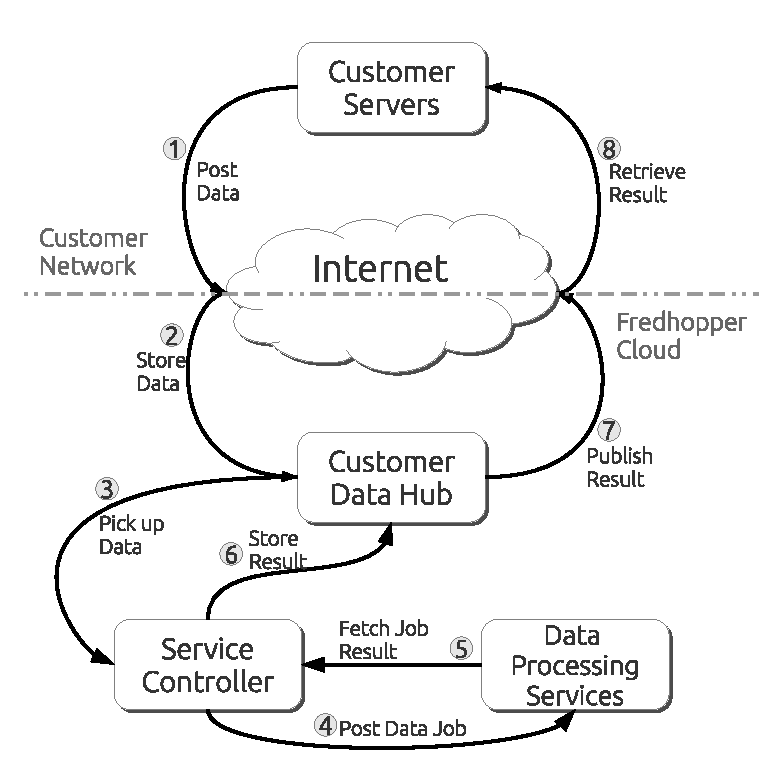
\includegraphics[scale=0.7]{images/DM}
\end{center}
% \vspace{-20pt}
\caption[Life cycle for data processing requests from customers]{Fredhopper's Controller life cycle for data processing requests from customers}
\label{ch05:fig:frh-dm}
% \vspace{-5pt}
\end{figure}
% \end{wrapfigure}

To orchestrate different services such as FAS or data processing, Fredhopper takes advantage of a service controller (referred to as Controller).
The Controller manages different service installations for each customer.
For instance, a customer can submit their data along with a processing request to their data hub server.
The Controller then picks up this data and initiates a data processing job, usually in the cloud.
When the data processing is complete, the result is published to the customer environment and becomes also available through FAS services.
Figure \ref{ch05:fig:frh-dm} illustrates this example scenario.

The Controller provides a simple client API for customers to develop applications that use Fredhopper services.
Essentially a data job request consists of three major steps:
\begin{enumerate}
 \item Prepare the data , upload it to the customer data hub and receive a data identifier.
 \item Specify the data processing: reindexing, updating or loading data. Such actions are called \emph{trigger}s.
 \item Collect the results of a trigger and decide how to use them.
\end{enumerate}
%For modularity and loosely coupling, a data identifier is not \emph{strictly} required to create a new trigger.
%There are triggers that actually require no data to be initiated while others do.
The customer is required to have the appropriate data identifier before executing a new trigger. In fact, the customer application
is supposed to use the proper sequence of operations from the API.

In this case study, we examined and measured how JMSeq can help customers improve their usage of client API for data processing; 
i.e. verify data processing triggers and notify customers as soon as they occur.
We used ``rebuild'' and ``update'' triggers in this experiment based on customer environment data from the period of February 2013
\footnote{Fredhopper data in this research is confidential due to privacy protection of customers.}.
In this experiment, we measured the following:
\begin{enumerate}
\item Using the log files, we replayed the triggers twice with different settings.
\item In one setting, we replayed the original customer data processing trigger.
\item In the other setting, we replayed the original customer data processing that was wrapped with JMSeq verification.
\item In each setting, we measured the number of \emph{successful} and \emph{failed} triggers. 
A successful trigger is one for which data processing completes and the result is reported back to customer data environment.
\end{enumerate}

Figure \ref{ch05:fig:frh:cs} presents the measurements for each setting without using JMSeq and with using JMSeq for both rebuild and update triggers.
The measurements were based on an estimated number of 30300 triggers in the same period.
Each figure shows the influence of using JMSeq for the data processing task.
On the left, measurements shows that JMSeq verification for rebuilding the catalog helps to decrease failures by 15\% if using JMSeq verification.
On the right, measurements shows that JMSeq verification has less influence to improve update process as it natually involves less erroneous data because of smaller data size in update triggers.

\begin{figure}
\begin{center}
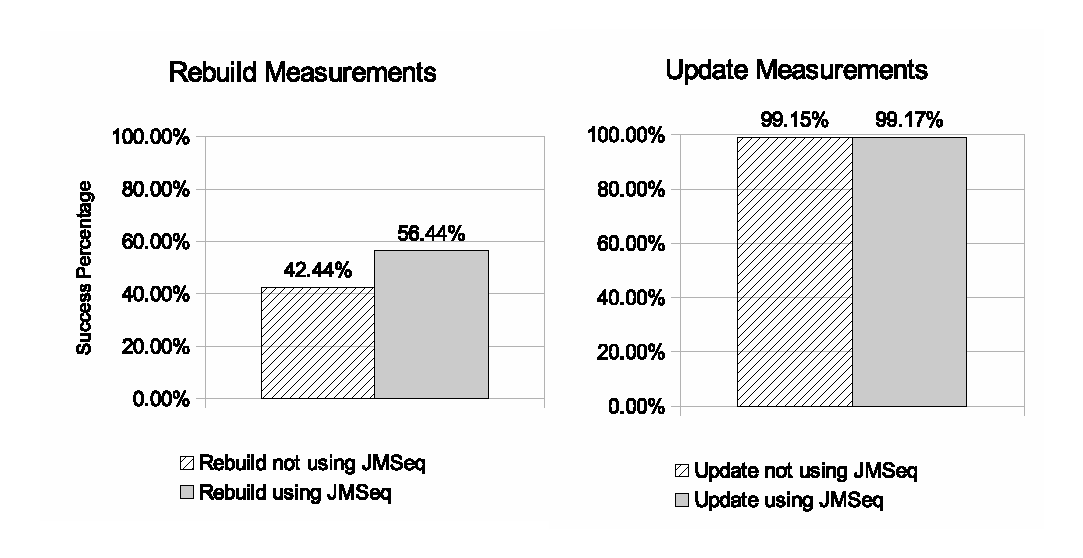
\includegraphics[scale=0.72]{images/frh-case-study-summary-rev2}
\caption[Comparison of measurements using JMSeq at Fredhopper]{Result of experiment measurements without and with using JMSeq on Fredhopper Client API directed with live environment data from customers.}
\label{ch05:fig:frh:cs}
\end{center}
\end{figure}

%In this case study, we apply JMSeq to a sample customer application to verify that the methods of the FAS API are used in the correct order.
%We \emph{cannot} expect to have the source code for the application.
%However, since the customer uses Fredhopper Controller API, we can expect what API is used from Fredhopper services.
Next we present the case study in code listings in which JMSeq monitors calls to methods of the Controller API.
The runtime environment stops as soon as an incorrect sequence of calls is detected.
%Thus, the customer is prevented from further steps.
%Such prevention can have significant impact on the customer's business.
%A customer may create a considerable number of triggers on a daily basis.
%The result of each trigger has a direct influence on the end users of the customer.
%Being able to prevent risky or erroneous product catalog updates substantially helps a customer to plan the services they deliver to the end users.

%Fredhopper Controller exposes an interface to prepare data, submit the data and then receive/collect the data job results.
\lstset{language=java}
\begin{lstlisting}[label=lst:frh:datadispatcher, caption=Controller Data Dispatcher Interface API]
interface DataDispatcher {
   Data create(Object object);
   Future<?> dispatch(String dataId);
   Future<?> dispatch(Data oid, String dataId);
}
\end{lstlisting}

The relevant part of the API of the Fredhopper Controller is presented in Listing \ref{ch05:lst:frh:datadispatcher}.
Customer applications use the interface to create a data object reference (using the \smalltt{create(Object)} method) and then use the created data reference to start a data job (using the overloaded \smalltt{dispatch} method, which has an optional \smalltt{Data} parameter).
Note that the dispatch method allows for two different uses by the customer, for instance in Listing~\ref{ch05:lst:frh:c1} the data job to be executed performs only a rebuild of the customer's product catalog and as such does not need to have a data reference.
\lstset{language=java}
\begin{lstlisting}[label=lst:frh:c1, caption=A use case with no data requirement]
class CustomerApp {
   public void rebuildCatalog() {
      Future<?> result = 
         dispatcher.dispatch("reindex");
      // further processing of result
   }
}
\end{lstlisting}
If the customer needs to update their catalog with new products, then first a data reference is created. This reference is used to initiate a data job, as described in Listing \ref{ch05:lst:frh:c2}.
\lstset{language=java}
\begin{lstlisting}[label=lst:frh:c2, caption=A use case with data requirement]
class CustomerApp {
   public void updateCatalog(Catalog catalog) {
      Data data = dispatcher.create(catalog);
      Future<?> result = 
         dispatcher.dispatch(data.getId(), "update");
      // further processing of result
   }
}
\end{lstlisting}

Note that we cannot expect to have the source code of the above listings.  To verify the correct use of the Fredhopper Controller API
with JMSeq we can create a \smalltt{CustomerAppDriver} class which calls the \smalltt{CustomerApp} methods and monitors the subsequent
method calls.  The expected usage of the API of the two scenarios above is described by the SequencedMethod annotations in Listing~\ref{ch05:lst:frh:c3}.
If the \smalltt{CustomerApp} does not behave as expected, the verifier detects an error.

\lstset{language=java}
\begin{lstlisting}[float=t,label=lst:frh:c3, caption=How to verify Fredhopper API usage]
@SequencedObject
class CustomerAppDriver {

   @SequencedMethod(
      "{call(* nl..CustomerApp.rebuildCatalog()" +
      "[{call(* nl..DataDispatcher.dispatch(String))}]}")
   public void verifyRebuildCatalog() {
      // initiate the customer application
      app.rebuildCatalog();
      // finalize verification
   }

   @SequencedMethod(
      "{call(* nl..CustomerApp.updateCatalog(Catalog)" +
      "[{call(* nl..DataDispatcher.create(Object)}" + 
      "{call(* nl..DataDispatcher.dispatch(Data, String))}]}")
   public void verifyUpdateCatalog(Catalog catalog) {
      // initiate the customer application
      app.updateCatalog(catalog);
      // finalize verification 
   }
}
\end{lstlisting}

%Figure \ref{ch05:fig:frh:cs} shows how using JMSeq in an evaluation environment for the customers detects violations and
%improves the usage of Controller API and eventually affects the success rate of triggers for customers.

% \newpage
\subsection{Discussion} \label{ch05:sec:discuss-jmop}

We use JavaMOP \cite{chen_rosu_jmop,chen_rosu_mop,MOP} for the same case study from Fredhopper. 
Listing \ref{ch05:lst:frh:jmop} shows a JavaMOP script to describe the same verification goal.

\lstset{language=[AspectJ]Java, morekeywords={suffix, event,ere, CFG, @fail, @match, __RESET}} 
\begin{lstlisting}[label=lst:frh:jmop, caption=Fredhopper case study with JavaMOP]
UpdateCatalog(Catalog catalog) {
   event create_data before(DataDispatcher d):
      call(* DataDispatcher.create(..)) && target(d) {}

   event dispatch_data before(DataDispatcher d):
      call(* DataDispatcher.dispatch(..)) && target(d) &&
      cflow(dispatch_data) {}

   ere: (create_data dispatch_data)

   @fail { __RESET; }
}
\end{lstlisting}
JavaMOP uses aspect-orientation and Java bytecode instrumentation.
Using aspects (e.g., as in AspectJ \cite{kiczales_aspectj}) means that the eventual customer application bytecode is instrumented.
The question is \emph{how can it be proved that JavaMOP does not have any influence on the application?}
%Moreover, JavaMOP requires source code of the application to generate the required AspectJ sources.
If the customer is not willing to cooperate in such a process, the system cannot be monitored with JavaMOP.
%because they believe the risk of having an impact on the eventual software cannot be controlled if it happens.
JMSeq on the other hand does not change the source- or bytecode, because JMSeq runs on a different JVM as the one running the customer application.
%uses Java annotations to express runtime verification goals.
%By definition, a Java annotation is a syntactic metadata that is carried either at source level or runtime level.
%Java annotations have no effect on the logic of the executing Java application.
%However, if available at runtime, the Java application has the opportunity to use such metadata for orthogonal purposes aside main execution of the application.
%Moreover, JMSeq runs a in a separate JVM from the one that is actually running the Java application.
%Therefore, JMSeq introduces a highly safe approach for runtime verification.
%Since the customer application is affected in no way by JMSeq, they have more inclination to use such approach to verify their applications.

\section{Performance Results} \label{ch05:sec:results}

In this section, we present performance measurements of JMSeq and other techniques to verify a program.
We choose a problem that has been studied in the context of JavaMOP \cite{chen_rosu_jmop} to provide a reference for comparison.

The example verifies the correct use of \smalltt{java.util.Iterator}.
Originally, the interface introduces two major methods: \smalltt{hasNext()} and \smalltt{next()}. 
The first one checks whether there are still elements in the sequence that can be visited and the second one gives out the next element in the sequence and moves forward.
An invocation of \smalltt{next()} presumes that it succeeds an invocation of \smalltt{hasNext()}.
Otherwise, an invocation of \smalltt{next()} may lead to an exception.

We use JMSeq to verify an example code for this scenario. 
We use the code snippet displayed in Listing \ref{ch05:lst:jmseq-iter} that uses JMSeq annotations to express the correct usage. 
In the code, we use a variable \smalltt{count} to control the number of times \smalltt{hasNext()} is called before there is a call to \smalltt{next()}. 
This example always passes the JMSeq verification with success. 
For performance measurements, we study the ``correct'' use of the example while verification of wrong usages are also possible. 
\lstset{language=Java}
\begin{lstlisting}[label=lst:jmseq-iter, caption=Iterator usage with
JMSeq Annotations]
   @SequencedMethod(
     value = "{call(* java..Vector.iterator())}$"
         + "{call(* java..Iterator.hasNext())}$"
         + "{call(* java..Iterator.next())}", 
        allowExceptions = false)
   public void visitAllElements() {
      Iterator<Integer> i = v.iterator();
      for (int k = 0; k < count && i.hasNext(); ++k) {
         i.hasNext();
         i.next();
      }
   }
\end{lstlisting}

In the following, we provide certain measurements from executions of JMSeq for the example above for different values of \smalltt{count} in \smalltt{\{10000, 15000, 20000, 30000, 50000, 100000, 200000\}}. 
We use VisualVM tool that is a standard profiling and performance measurement tool packaged with standard Java development packages.

We measure the execution time of the following cases:
\begin{description}
\item[original.] We execute the original program and measure the execution time of the program with the above \smalltt{count} values.
\item[instrumented.] We use a technique that uses instrumentation such as JavaMOP \cite{chen_rosu_jmop} and apply it to the program and measure the execution time the same.
\item[original{\textbackslash}JMSeq.] We execute the original program and monitor it by JMSeq. We measure the execution time of the original program while being verified by JMSeq.
\end{description}

Figure \ref{ch05:fig:jmseq-performance} displays how different cases compare to each other regarding the execution time. 
As expected, the original program execution has the lowest execution time.
Since techniques based on instrumentation modify the bytecode of the program, this adds to the execution time of the program.
The figure shows that compared to instrumentation techniques, JMSeq adds a lower overhead.

\begin{figure}
\begin{center}
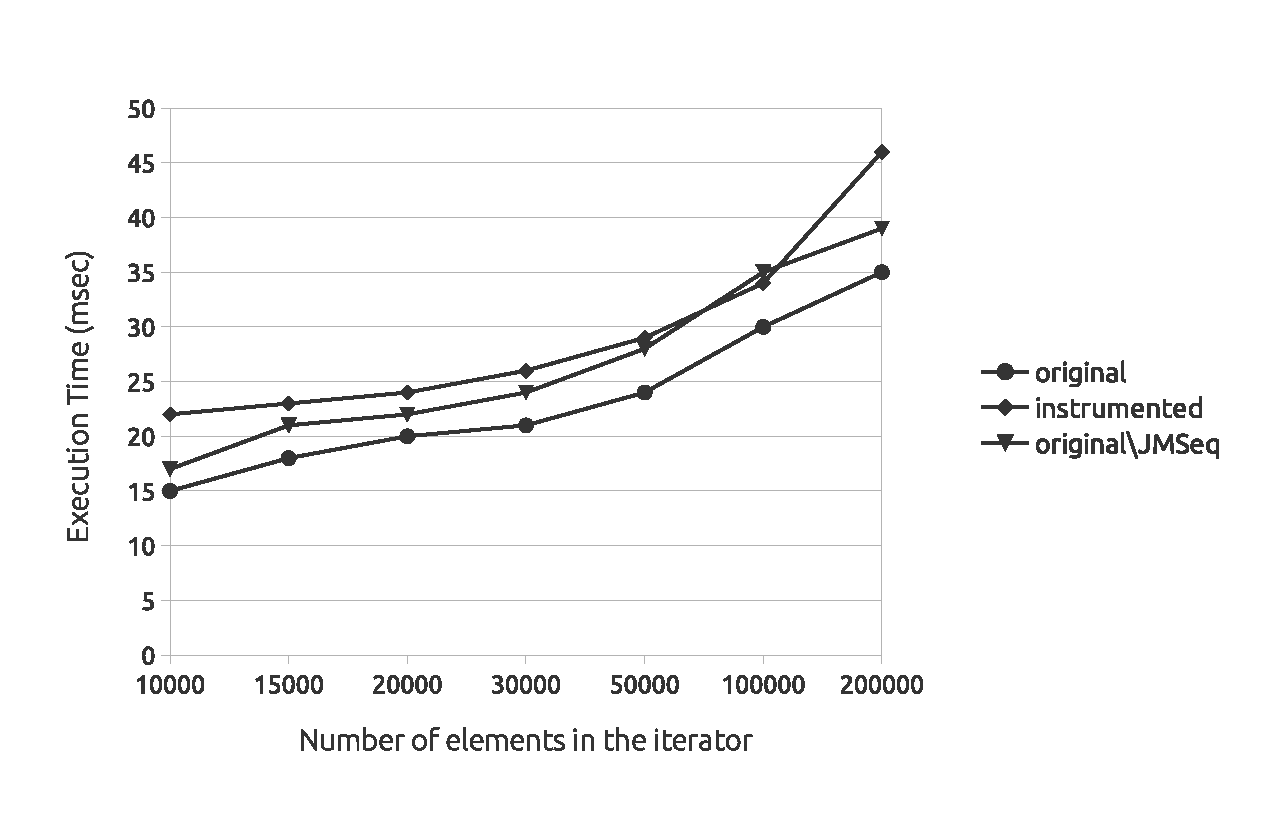
\includegraphics[scale=0.55]{images/perf}
\caption[Comparison of different techniques with JMSeq]{Comparison of different techniques applied to the same program. 
In this figure, ``original'' denotes the original program that is measured for execution time;
``instrumented'' denotes using a technique such as JavaMOP that uses instrumentation for verification;
 and ``original{\textbackslash}JMSeq'' denotes the measurement of the execution time for the program apart from times for JMSeq.}
\label{ch05:fig:jmseq-performance}
\end{center}
\end{figure}

We use the performance results here to argue that the technique used by JMSeq is more suitable to verify applications that are mission-critical or operate on a high load.
Experience shows that, under high load, issues start to emerge that do not exist under normal operational situations.
In such circumstances, the application provider is very likely to look for methods to verify and detect problems.
And yet, they need to make sure that the application remains at least at the same level of execution and performance.
Moreover, the fact that JMSeq runs in a separate JVM increases the safety of our approach, since
JMSeq can be used from even a remote machine to verify a program, without the slightest influence on the resources that run the target program.

% JMSeq process of verification consists of two major activities in the context of performance and profiling:
% \begin{description}
% \item [Execution data model] that first receives the event
% from JPDA and the target JVM and prepares an execution data model for
% JMSeq verification.
% \item [Verification] that uses the execution data model to verify the
% current event based on the annotations, history of executions and the
% next possible execution.
% \end{description}

% \begin{table}[t]
% \begin{center}
% \begin{tabular}{|c|c|c|c|}\thickhline
% \texttt{count} & Total Time (msecs) & Invocations & Single Invocation
% Time \\ \thickhline
% 10,000 & 798 & 28751 & 0.0278 \\
% 15,000 & 1240 & 48204 & 0.0257 \\
% 20,000 & 1830 & 73470 & 0.0249 \\
% 30,000 & 2651 & 109909 & 0.0241 \\
% 50,000 & 4605 & 200010 & 0.0230 \\
% 100,000 & 9873 & 400010 & 0.0247 \\
% 200,000 & 19607 & 800010 & 0.0245 \\ \thickhline
% \end{tabular}
% \end{center}
% \caption{Execution data model performance results with JMSeq}
% \label{ch05:tab:results-handleevent}
% \end{table}

% Using VisualVM, we observed different measurements for both
% execution data model and verification. Please also
% note that the verification time is by nature different from
% execution time; i.e. we do not measure the execution time of the
% underlying application but we measure the time JMSeq takes to verify the
% executions in the application and then either allow or disallow the
% execution. In addition, we measure three metrics for the performance:
% total time for each JMSeq activity, number of invocations of each JMSeq
% activity, and a computed time for a single JMSeq activity. Table
% \ref{ch05:tab:results-handleevent} summarizes the performance results for
% execution data model and Table \ref{ch05:tab:results-verify} summarizes the
% same facts for verification. 

% \begin{table}[t]
% \begin{center}
% \begin{tabular}{|c|c|c|c|}\thickhline
% \texttt{count} & Total Time (msecs) & Invocations & Single Invocation
% Time \\ \thickhline
% 10,000 & 1120 & 28751 & 0.0390 \\
% 15,000 & 1698 & 48204 & 0.0352 \\
% 20,000 & 2558 & 73470 & 0.0348 \\
% 30,000 & 3504 & 109909 & 0.0319 \\
% 50,000 & 6388 & 200005 & 0.0319 \\ 
% 100,000 & 12753 & 400005 & 0.0319 \\
% 200,000 & 25805 & 800005 & 0.0323 \\ \thickhline
% \end{tabular}
% \end{center}
% \caption{Verification performance results with JMSeq}
% \label{ch05:tab:results-verify}
% \end{table}

% The results show that JMSeq has a \textit{linear} co-relation to the
% number of invocations that it needs to verify (Figure
% \ref{ch05:fig:jmseq-performance}). In this example, we set
% up \smalltt{count} to increase in an ``exponential'' way, thus, JMSeq
% performance also is affected in an exponential manner pertaining to the
% linear co-relation to \smalltt{count}. In addition, it is worthwhile
% to note that generating the events from JPDA is another concern. In
% this regards, we tested different \emph{standard} implementations of
% JPDA including the standard reference implementation \cite{JPDA_Home}
% and Eclipse JDT implementation \cite{eclipse_jdt} in which both
% converging to the same results. 


% Since JMSeq and the target Java program run in different JVMs, a future
% work for improving the performance of runtime verification is to run
% these JVMs in parallel, for example using a multi-core processor.
% Such a decoupling is possible because JMSeq is based on annotations
% that leave the execution of the original Java program intact.
% We expect a good speed-up because the communication between these two
% JVMs is limited to a one-way (and possibly asynchronous) sending of
% events.

\section{Related Work} \label{ch05:sec:relworks}

JML \cite{leavens_baker_ruby_jml_design} provides a robust and rigorous grounds for specification of behavioral checks on methods. 
Although JML covers a wide range of concerns in assertion checking, it does \textit{not} directly address the problem of method call sequence specification  as it is more directed towards the reasoning about the state of an object. 
JML is rather a comprehensive modeling language that provides many improvements to extensions of Design by Contract (DBC) \cite{dbc} including jContractor \cite{jcontractor} and Jass \cite{jass}.

In \cite{yoonsik_ash_mscs}, taking advantage of the concept of
\textit{protocols}, an extension to JML is proposed that provides a syntax for
method call sequences (protocols) along with JML's functional specification
features. Through this extension, the developer can specify the methods' call
sequence through a \textsl{call sequence clause} in JML-style meta-code. In the
proposed method, the state of a program is modeled as a ``history'' of method
calls and return calls using the expressiveness of regular expressions; thus, a
program execution is a set of ``transitions'' on method call histories. The
verification takes place when the execution history is simulated using a finite
state machine and checked upon the specified method call sequence clause.

JML features have been equivalently implemented with AspectJ constructs
\cite{jml_aspects}, using aspect-oriented programming \cite{kiczales_aspectj}.
The authors of this work propose AJMLC (AspectJ JMLC), which integrates AJC and JMLC into a single compiler
so that instead of JML-style meta-code specifications, the developer writes 
\textsl{aspects} to specify the requirements. 

In \cite{stijn} an elegant extension of JML with histories is presented.
Attribute Grammars \cite{DBLP:journals/mst/Knuth68} are used as a formal
modeling language, where the context-free grammar describes properties of the
control-flow and the attributes describe properties of the data-flow, providing
a powerful separation of concerns. A runtime assertion checker is
implemented. Our approach differs in several respects. The
implementation of their runtime checker is based on code
instrumentation. Additionally, they use local histories of objects,
so call-backs can not be modeled. However, the behavior of a stack
can be modeled in their approach (and not in ours), since their
specifications are not regular expressions but context-free languages.

In the domain of runtime verification, Tracematches \cite{tracematches} enables the
programmer to specify events in the execution trace of a program that could be specified 
with ``the expressiveness'' of a regular pattern. The specification is done with 
AspectJ pointcuts and upon a match the advised code is run for the pointcut.
Along the same line, J-LO \cite{bodden_jlo} is a tool that provides temporal assertions in
runtime-checking. J-LO shares similar principles as Tracematches with differences 
in specifications using linear time temporal logic syntax.

Additionally, Martin et al. propose PQL \cite{martin_livshits_lam_pql} as a 
program execution trace query language. It enables the programmer to express queries 
on the execution events of objects, methods and their parameters. PQL then takes 
advantage of two ``static'' and ``dynamic'' checkers to analyze the application. The 
dynamic checker instruments the original code to install points of ``recovery'' and
``verification'' actions. The dynamic checker also translates the queries into
state machine for matching criteria. The set of events PQL can deal with
includes method calls and returns, object creations and end of program among
others. Accordingly, generic logic-based runtime verification frameworks are
proposed as in MaC \cite{java_mac}, Eagle \cite{eagle}, and PaX (PathExplorer)
\cite{pax} in which monitors are instrumented using the specification based on
the language specific implementations.

Using runtime verification concepts, Chen and Rosu propose MOP
\cite{chen_rosu_mop,MOP} as a generic runtime framework to verify programs
based on monitoring-oriented programming. As an
implementation of MOP,
JavaMOP \cite{chen_rosu_jmop} provides a platform supporting a large part of
runtime JML features. Safety properties of a program are specified and 
inserted into the program with monitors for runtime verification. Basically,
the runtime monitoring process in MOP is divided into two orthogonal
mechanisms: ``observation'' and ``verification''. The former stores the desired
events specified in the program and the latter handles the actions that are
registered for the extracted events. Our approach follows the same idea as MOP,
but it does not use AOP to implement it. Another major
difference is in the specifications part. MOP specifications are  generic in
four orthogonal segments: logic, scope, running mode and event handlers.  Very
briefly, the \textit{scope} section is the fundamental one that defines and
specifies the parts of the program under test. It also enables the user to
define desired events of the program that need to be verified. The
\textit{logic} section helps the user specify the behavioral specification of
the events using different notations such as regular expressions or
context-free grammars. The \textit{running mode} part lets the user specify
what is the running context of the program under test; for instance, if the
test needs to be run per thread or in a synchronized way. And, \textit{the
event handlers} section is the one to inject customized code of verification or
logic when there is a match or fail based on the event expression logic.
In Section \ref{ch05:sec:discuss-jmop}, we discussed how JMSeq contrasts with JavaMOP and similar approaches.

% In Listing \ref{ch05:lst:sample_mop} we show an example of JavaMOP code with ERE
% logic for the two specifications given in Figure \ref{ch05:fig:seq-spec}.

% \lstset{language=[AspectJ]Java, morekeywords={suffix, event,ere, CFG, @fail, @match, __RESET}} \begin{lstlisting}[label=lst:sample_mop, caption=Sample JavaMOP Specification using CFG logic] // Case 1
% SampleCase1(Main m) {
%  event method_m_a before(A a):
%     call(* A.m_a(..)) && target(a) {}

%  event method_m_b before(B b):
%     call(* B.m_b(..)) && target(b) && 
%     cflow(SampleCase1_method_m_a) {}

%  event method_m_c before(C c):
%     call(* C.m_c(..)) && target(c) && 
%     cflow(SampleCase1_method_m_a) && 
%     cflow(SampleCase1_method_m_b) {}
   
%  ere: (method_m_a method_m_b method_m_c)*
   
%  @fail {
%     System.err.println("Invalid Execution");
%     __RESET;
%  }     
% }

% // Case 2
% SampleCase2(Main m) {
%  event method_m_a before(A a):
%     call(* A.m_a(..)) && target(a) {}

%  event method_m_b before(B b):
%     call(* B.m_b(..)) && target(b) && 
%     cflow(SampleCase1_method_m_a) {}

%  event method_m_c before(C c):
%     call(* C.m_c(..)) && target(c) && 
%     cflow(SampleCase1_method_m_a) && 
%     !cflow(SampleCase1_method_m_b) {}
   
%  ere: (method_m_a method_m_b method_m_c)*
      
%  @fail {
%     System.err.println("Invalid Execution");
%     __RESET;
%  }     
% }
% \end{lstlisting}

% The code snippet presented in Listing \ref{ch05:lst:sample_mop} is one of
% several ways to express the problem described in Figure
% \ref{ch05:fig:seq-spec}. JavaMOP allows the use of AspectJ language to
% define the scope of the program points to be verified. This may look
% advantageous since the programmer can use different syntax in
% AspectJ. However, it leads to low-level specification of control flow
% using AspectJ in addition to JavaMOP logic section syntax. In
% particular, the \smalltt{cflow} keyword in the event definitions
% (scope section), already specifies the logic. In contrast, JMSeq allows
% for purely declarative specification language which completely captures
% the operational behavior using regular expressions. For instance,
% in Section \ref{ch05:sec:spec}, we used
% %\begin{flushleft}
% %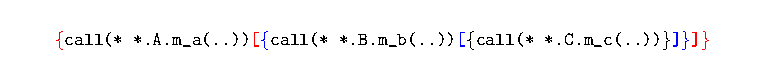
\includegraphics[scale=1]{grammar-sample-usage-1}
% \begin{alltt} 
\centering\small{\color{red}\{}call(* *.A.m_a(..)){\color{red}[}{\color{blue}\{}call(* *.B.m_b(..)){\color{blue}[}\{call(* *.C.m_c(..))\}{\color{blue}]}{\color{blue}\}}{\color{red}]}{\color{red}\}}
\end{alltt}

% %\end{flushleft}
% and
% %\begin{flushleft}
% %\includegraphics[scale=1]
% \begin{alltt} 
\centering\small{\color{red}\{}call(* *.A.m_a(..)){\color{red}[}\{call(* *.B.m_b(..))\}{\color{red}]}{\color{red}[}\{call(* *.C.m_c(..))\}{\color{red}]}{\color{red}\}}
\end{alltt}

% %\end{flushleft}
% to specify the same program in Figure \ref{ch05:fig:seq-spec}.
% Another major difference between JMSeq and JavaMOP is the use of
% annotations versus instrumentation as already discussed in Section
% \ref{ch05:sec:intro}.

% It is interesting to note that both MOP specifications have \textit{the same
% ERE expression}. This is because JavaMOP has separated logic and scope
% specification from event handling. The difference in monitoring is
% obtained by the different usage of the command {\small\texttt{cflow}} in the
% scope section. This command is an AspectJ construct to control the context of
% the execution when running some code inside a method
% \cite{kiczales_aspectj}. Seemingly, even though JavaMOP claims to
% support a separation of concerns, the event definitions are mixed with
% behavioral specification in aspects declarations such as
% \smalltt{cflow}. In contrast, JMSeq provides all the specification
% through the annotations that are used by the programmer user.


\section{Conclusion and future work} \label{ch05:sec:conclusion}

We proposed JMSeq, a framework for specifying sequences of possibly nested method calls using Java annotations. 
The sequences do not only consist of method names, but may contain information such as object caller and callee, and distinguish overloaded methods. 
JMSeq uses Java Platform Debugger to monitor the execution of a component-based system in Java. 
Monitoring is divided into two phases: observing the events in the program and verifying them at runtime against the local specifications provided through annotated methods. 
JMSeq does not use \emph{any} form of instrumentation; neither source level nor bytecode level.
Moreover, JMSeq provides a simple way to express exceptions and verify them in the execution of the target application. JMSeq is integrated with JUnit.
We presented a case study from Fredhopper distributed cloud services in the domain of e-commerce and marketing. 
Moreover, we provided a set of performance results for JMSeq in different settings for program execution and runtime verification.

JMSeq is a novel approach to runtime verification of software using code annotations. 
The approach is especially suitable for runtime component-based verification. 
We improved the execution data model of JMSeq using optimization techniques such as in-memory object caches with indices.
In the context of event processing, we examined different implementations of JPDA and JDI standards (e.g. using Eclipse platform \cite{eclipse_debug_platform}) and it showed part of the optimization is out of our reach. 
We used VisualVM, a standard Java profiling tool, to measure and discuss the performance of JMSeq.

A future line of work consists of porting JMSeq to multi-core platforms. 
Concurrent and distributed software introduces new challenges for runtime verification of applications. 
In a concurrent setting, objects interact with each other from different threads of execution (which may optionally involve synchronization and locking events).
JMSeq should be able to verify such objects in different threads and consider how synchronization and locking may affect the runtime or flow of an application.
In a distributed context, application objects are located in (physically) remote JVM instances.
In such scenarios, JMSeq needs to load or observe a topology of the involved JVMs and their objects to be able to verify the application for correct sequences of method calls.

We plan to extend JMSeq by providing native features such as mock \cite{frank:mock} implementations in case parts of the system are unavailable.
JMSeq may provide better integration for mocking parts of the system that are not implemented or not available.
Such features will be especially useful in the context of integration testing and verification.
At the time of integration, not all components of the system may be available and complete; and yet, the application should be verified in the parts that are complete.
In comparison with runtime checking, another line of future work can be to extend JMSeq to support static verification of protocols (using approaches as in Copilot \cite{copilot}). 

% Moreover, in another direction, the testing framework can even take control of the
% underlying program execution for further checks or verification. 
% In other words, method call sequence specifications may also be used in the pre-conditions of a method such that a method is executed only if it is allowed in the high-level specification. 

Finally, we plan to  extend the specification language to a context free language. 
This is in fact simple as JMSeq already implements a simple form of pushdown automata to recognize the call-return structure of Java.
In fact, Java is expressible by a restricted form of deterministic pushdown automata, called  visibly pushdown automata \cite{Alur_abstractvisibly}, where push and pop correspond to call and return, respectively. 

% Another potential area of improvement is the data model used
% by JMSeq. Currently
% it overlaps with the event model that JPDA provides when publishing the
% registered events in JVM. The resulting overhead is rather expensive.
% Optimization will allow, for example, to store only the minimal necessary
% information providing a faster indexing for the retrieval of the events.
% Further performance improvement can be obtained by better exploiting the
% connections between JPDA and JVM. For example, there are tools such as Eclipse
% Debug Platform \cite{eclipse_debug_platform} that provide extensive
% facilities through JPDA with high performance. Currently, in JMSeq, it is the
% standard JVM that runs the program and publishes the events that are
% interesting to JMSeq for further verification for which, in turn, JMSeq uses a
% simple state machine to verify the executing events. 

% \paragraph{Acknowledgments}
% We thank the referees for their comments and Michiel Helvensteijn for 
% the helpful discussion.

% \bibliographystyle{abbrv}
% \bibliography{references}

% \end{document} 
